\documentclass[a4paper,11pt]{report}
%\documentclass[a4paper,12pt]{article}
\usepackage[backend=biber,sorting=ydnt,maxnames=18,giveninits=true,labelnumber=true,defernumbers=true]{biblatex}
%\usepackage[backend=biber,sorting=ydnt,maxnames=18,giveninits=true,labelnumber=true,defernumbers=true]{biblatex}
%\usepackage[backend=biber,sorting=ydnt,maxnames=18,giveninits=true]{biblatex}
%\usepackage[bibstyle=publist]{biblatex}
\usepackage{xstring}
\usepackage{url}
\usepackage{booktabs}
\usepackage{hyperref}
\usepackage{color}

\usepackage{titlesec}
\definecolor{gray75}{gray}{0.75}
\newcommand{\hsp}{\hspace{20pt}}
\titleformat{\chapter}[hang]{\huge\bfseries}{\thechapter\hsp\textcolor{gray75}{|}\hsp}{0pt}{\huge\bfseries}
\titlespacing*{\section}{0pt}{6pt plus 1pt minus 0.5pt}{3pt plus 0.5pt}
\titlespacing*{\chapter}{0pt}{12pt plus 1pt minus 0.5pt}{6pt plus 0.5pt}
\titlespacing*{\subsection}{0pt}{6pt plus 1pt minus 0.5pt}{3pt plus 0.5pt}
%\titlespacing*{\subsection}{0pt}{5.5ex plus 1ex minus .2ex}{4.3ex plus .2ex}

\titlespacing*{\paragraph}
{0pt}{3pt plus 1pt minus 0.5pt}{3pt plus 2pt minus 0.5pt}

\usepackage{enumitem}
\setlist{nosep}

\usepackage{tcolorbox}

\usepackage{fontspec}
\setmainfont{Cambria}
\setsansfont{Calibri}

%\setlength{\itemsep}{0pt plus 1pt}
%\setlength{\itemsep}{0pt}
%\setlength{\topsep}{0pt}
\setlength{\parskip}{3pt plus 0.5pt minus 0.5pt}
%\setlength{\beforeskip}{3pt}


\usepackage[scale=0.85]{geometry}

\geometry{
 a4paper,
 total={170mm,257mm},
 left=20mm,
 top=20mm,
 }

%\assignrefcontextkeyws[labelprefix=C]{C}
%\assignrefcontextkeyws[labelprefix=J]{J}

\addbibresource{bib/varrodan.bib}
\addbibresource{bib/external.bib}
%\addglobalbib{bib/external.bib}

%\assignrefcontextkeyws[labelprefix=C]{C}
%\assignrefcontextkeyws[labelprefix=J]{J}

\renewcommand*{\mkbibnamegiven}[1]{%
%\ifpartannotation{family}{self}{\textbf{#1}}{#1}}
\ifpartannotation{family}{self}{\ifcategory{mcgill}{\mkbibbold{\underline{#1}}}{\textbf{#1}}}{#1}}

\renewcommand*{\mkbibnamefamily}[1]{%
\ifpartannotation{family}{student}{#1\textsuperscript{*}}{%
%\ifpartannotation{family}{self}{\textbf{#1}}{#1}}}
\ifpartannotation{family}{self}{\ifcategory{mcgill}{\mkbibbold{\underline{#1}}}{\textbf{#1}}}{#1}}}

\usepackage{fancyhdr}
\pagestyle{fancy}\lhead{Tenure Dossier} \rhead{August 2019}
\chead{{\bf Dániel Varró}} \lfoot{} \rfoot{\bf \thepage} \cfoot{}

%\title{Teaching Portfolio}
%\author{D\'aniel Varr\'o}
%\date{August 2019}

\DeclareRefcontext{bref}{labelprefix=B}
\DeclareRefcontext{jref}{labelprefix=J}
\DeclareRefcontext{cref}{labelprefix=C}
\DeclareRefcontext{wref}{labelprefix=W}
\DeclareRefcontext{oref}{labelprefix=O}
\DeclareRefcontext{eref}{labelprefix=E}
\DeclareRefcontext{iref}{labelprefix=I}
%\DeclareRefcontext{extref}{labelprefix=X,sorting=none}
\DeclareRefcontext{extref}{sorting=none}
\DeclareBibliographyCategory{own}
\DeclareBibliographyCategory{mcgill}

\begin{document}

\chapter{Personal Statement}

After a successful academic career pursued in Hungary at the Budapest University of Technology and Economics where I got tenure in 2009 and promoted to a full professor in 2014, I joined the Department of Electrical and Computer Engineering at McGill University as a full professor in August 2016. Since 2015, I have held a research chair position in Hungary leaing a research program on cyber-physical systems as part of the prestigious and highly selective MTA Lendület program. 
This is an annually awarded in Hungary with only 12-15 researchers across all disciplines, and with only three past awardees in computer science since the foundation of the program in 2009. 

While this dossier dominantly presents details of my achievements after joining McGill University, I also provide a brief summaries about the pre-McGill period of my career. Furthermore, as a unique aspect of my research portfolio, I initiated and led an international research program involving more than 10 PhD students and several master's students both from Canada and Hungary.

\paragraph{Research.}
My main research area is \emph{model-based software and systems engineering} aiming for the design, analysis, optimization or deployment of traditional safety-critical systems as well as smart cyber-physical systems (CPS). My research contributed precise and scalable graph-based software techniques as foundations of design-time and run-time tools used in domains like avionics, automotive and various Internet-of-Things (IoT) systems. Since joining McGill University, we managed to substantially advance the state-of-the-art by (1) introducing distributed graph queries for runtime monitoring, (2) developing a novel family of automated model generator for domain-specific graph models, and (3) proposing various techniques secure collaborative modeling. Major ongoing multidisciplinary research carried out at McGill University aims to support the digital multidisciplinary analysis and design optimization platform.

I have been continuously aiming to publish my research results at top scientific conferences and journals of model-driven engineering (my direct research area) or alternatively, at general software engineering venues. In my career, I have published 171 papers (34 since joining McGill) including 47 papers in peer-reviewed journals (10 at McGill), and 73 peer-reviewed conference papers (20 at McGill). I have published several papers at a large variety of major scientific venues of my research area including IEEE/ACM sponsored conferences of software systems such as e.g. MODELS, ICSE, ASE, ESEC/FSE and top journals (e.g. Software and Systems Modeling, IEEE Software, Software Tools on Technology Transfer, Science of Computer Programming, Information and Software Technology). My papers received over 6710 citations (according to \href{https://scholar.google.ca/citations?user=4Ya6dVoAAAAJ&hl=en}{GoogleScholar}) with a Hirsch-index of 43. As of today, I am the most cited software engineering researcher at McGill University.  

As a recognization of our research, \emph{seven papers} co-authored by my graduate students and myself received \emph{Best / Distinguished Paper Awards} at leading conferences (4x at MODELS, 1x at ASE 2011, 1x at CSMR-WCRE 2014 and 1x ETAPS 2018). Three of these papers were published after joining McGill University. Furthermore, \emph{two 10-year Most Influential Paper Awards} for our pioneering work on generic and meta-transformations (awarded at IEEE/ACM MODELS 2014) and benchmarking graph transformation tools (recognized at IEEE VL/HCC 2016).

I gave a total of 35 invited talks (10 talks since joining McGill) at international graduate schools, research seminars, at various companies (e.g. Ericsson, Embraer, Rockwell Collins) and research institutes (e.g NASA Jet Propulsion Lab, SRI International) - 10 of these talks were delivered after joining McGill. I was invited to give a keynote talk at leading software engineering conferences (CSMR 2012 and SOFSEM 2016), and a plenary talk at MODELS 2014 upon receiving the Most Influential Paper award. Moreover, I gave keynote talks at national conferences (CSER 2017 in Canada and CSCS 2016 in Hungary) and at numerous workshops. I gave a total of 9 talks and 4 tutorials at international summer schools.% (DSM-TP, SERENE, SENSUS). 

I was successful in securing competitive research funding on a Canadian, European and Hungarian level by acquiring an equivalent of over 4.5 million CAD for my own research. This includes competitive funding over 600,000 CAD in Canada (after joining McGill) along projects in the NSERC Discovery Grant program and the Collaborative Research and Development program with Siemens. Prior to succeeding as a Lendület research chair at the Hungarian Academy of Sciences, my ERC Starting Grant project CERTIMOT (in 2009) went through to the final round, and it was recommended for funding, but become out of budget, but it still received partial national funding later. I acted as the site leader (or research director at BME) of five collaborative European projects.% in the FP6 and FP7 framework in the field of service-oriented computing (SENSORIA), avionics (DIANA), evolving secure systems (SecureChange), transport (E-Freight) and scalable model-driven engineering (MONDO). 
I was the PI of industrial projects with Embraer, Ericsson and Nokia. I am a three-time recipient of the IBM Faculty Award.

\paragraph{Student supervision.}
I have been the main supervisor of 11 PhD students and a co-supervisor for 6 PhD students with 11 successful defenses up to now. Seven of those PhD students had a McGill affiliation (as a PhD student or as a graduate research trainee at McGill). I have also supervised 5 MEng students and 38 undergraduate students and at McGill University (with career total of 28 MSc/MEng students). 115 of my research papers have at least one student co-author I supervised or co-supervised (with 32 out of 34 papers after joining McGill). My graduate students successfully competed in various doctoral research competitions organized at top international conferences achieving twice a 1st prize and once a 3rd prize after I joined McGill. 
%Previously, I was selected as (the youngest ever) Distinguished Tutor, a bi-annual national prize requiring 10 years of successful tutoring. 
In 2017, I was the first ever recipient of the Csanád Imreh Award where a single award is given bi-annually to scientists in the field of computer science below the age of 41. 

\paragraph{Service.}
Since joining McGill University, I was invited to serve in various senior organizational roles at major international conferences, such as the program co-chair (SLE 2016, MiSE 2019), posters co-chair (ICSE 2019), program board member (MODELS 2016 and 2017), steering committee member (ICMT) or editorial board member (SoSyM, JOT). I served on the program committee of major international conferences of my field (including e.g. ICSE, MODELS, ICMT, ECMFA). At ICSE 2018, I received an \emph{ACM Distinguished Reviewer} award for my thorough reviews. I served as an external reviewer for various international projects and grants in 4 countries. Previously, I served as the program co-chair of FASE 2013, ICMT 2014, general chair of AGTIVE 2011 and STAF 2013, and the local organizing chair of ETAPS 2008 and EDCC-5, and served on the program committee of over 100 conferences and workshops.

At McGill University, I have served on 8 different committees for the ECE Department and 2 faculty-level working groups. For example, as a member of the Search Committee of the ECE Department in 2018 and 2019, I evaluated application packages of hundreds of applicants. Since 2018, I have been an elected representative of the Faculty of Engineering for the Council of Graduate and Postgraduate Studies (CGPS). In addition, I have been serving as an internal or external examiner for 5 PhD theses after joining McGill (with a career total of 24 PhD thesis reviews) in four different countries.


\paragraph{Teaching.}
Within the five courses I taught at McGill University, my most significant achievements were in the ECSE 321 Introduction to Software Engineering course where I successfully modernized the software technologies, brought in real customers for the complex software engineering project, redeveloped tutorials, and initiated the development of an autograder software for objectively evaluating technology assignments of students. Students are very supportive of my teaching style as 90\% of my instructor-specific course evaluation scores are over 4.0 (out of 5.0). Finally, I also gave 3 invited lectures and 2 tutorials at the international DSM-TP summer school. I also serve as the program director of the upcoming software engineering co-op program (expected to start in 2020) where undergraduate students will need to spend four compulsory internship terms at companies. In that role, I have been working on the key policies, guidelines, student and employer evaluation forms related to the co-op terms since Fall 2018.

%Teaching experience and course development. Since 2003, I have been involved in the development of 10 university courses on different levels (for BSc, MSc and PhD students) first at BME and then at McGill University. I was in charge of developing an undergraduate specialization on Systems engineering now an accredited curriculum at BME. I have been lecturing regularly for 70-120 on different levels (and occasionally for 200+ undergraduates). At McGill, I am the program director for the upcoming software engineering co-op program where undergraduates spend compulsory internships at companies as part of their curriculum. I am a co-author of a (Hungarian) textbook and I was an invited panelist at MODELS 2009 Educators’ Symposium. 

\paragraph{Experience in software industry.}
In 2013, I co-founded IncQuery Labs, an innovative Hungarian company, together with the first generation of my former PhD students (who are current executives of the company). I played a major role in acquiring the first large-scale projects e.g. with Ericsson and TeqBall and participating in its first European project OpenCPS. In 2016, the company received a 3rd place on the Deloitte Rising Star list as the fastest growing Hungarian company in Central Europe. In 2018, I was representing the company as part of the SysML 2.0 standardization in the Object Management Group. 

As further industrial experience, I was the founder and (until 2016) the main strategist of the open source VIATRA model query and transformation framework (used at Thales, Ericsson, NASA JPL, Airbus ThyssenKrupp Presta, several automotive tool vendors and in open tools like Capella, Artop or Papyrus) and a co-founder of MASSIF, a Matlab Simulink Integration Framework for Eclipse (used e.g. at INTECS, CEA, MapleSoft MBSE).  These projects started as research prototypes funded by research projects, and they gradually evolved to an industrial tool now maintained by IncQuery Labs Ltd.

%Previously, I was Vice President of Research at OptXware Ltd, a Hungarian spin-off company. I participated in a national project supporting the development of product family of service dependability and optimization.  After developing an Eclipse based toolkit for AUTOSAR, the company was partially acquired by a large international automotive company. I was one of the company representatives during the acquisition talks.

\chapter{Research Portfolio}
\label{sec:research-portfolio}
\lfoot{Research Portfolio} 
%\rfoot{Research Portfolio} 

%\begin{tcolorbox}[title=Summary of Excellence]
%My research primarily focuses on providing \emph{precise and scalable techniques} and \emph{software tools} used for engineering critical software-intensive systems with a recent focus on \emph{smart and safe cyber-physical systems} (CPS) deployed over decentralized, heterogeneous platforms. As the leader of an excellent research team with 15 PhD and 25+ Masters students I supervised or co-supervised, we received \emph{7x Best/Distinguished Paper Awards} at major peer-reviewed conferences of software engineering (3 of which since joining McGill). I also received \emph{two 10-year most influential papers} for past results achieved in my early career. My research papers received over 6700 citations yielding an h-index of 43. In the past 5 years, I was invited to deliver 6 keynote talks at international or national conferences or workshops, 10 talks at advanced schools, and 15+ talks at industrial events.
%
%\vspace{3pt}
%
%%\paragraph{A paragraph}
%Moreover, I have actively contributed to turn \emph{novel research results and prototype tools} first into \emph{industrial strength open source frameworks} then \emph{to innovative services and products} maintained by IncQuery Labs, a successful Hungarian company co-founded with my former graduate students and used by major international companies.
%% operating in the CPS domain.
%\end{tcolorbox}

\paragraph{Organization of research portfolio}

My career as an indepenent researcher consists two main stages. \textbf{Stage 1} is from 2004 when I started to independently supervise students at BME, which included 5 PhD students and numerous MSc students until 2014.
I successfully received a tenured position in 2009 and I was promoted to a full professor at BME in 2014, which I consider to be the end of this first stage. During these years, my research was primarily focusing on various model query and transformation techniques used in the model-based software and systems engineering for safety-critical systems. 

\textbf{Stage 2} (starting in 2015) has been carried out in a rather unique research environment.  I successfully applied to a professor position at the Department of Electrical and Computer Engineering at McGill University, and I also acquired a Hungarian prestigious and highly selective Research Chair position funded by the Hungarian Academy of Sciences to found the \href{https://mta.hu/lendulet/az-mta-lendulet-kutatocsoport-halozata-105402}{MTA-BME Lendület Cyber-Physical Systems Research Group} by \emph{initiating a new research program on designing and analyzing cyber-physical systems}. Since I got permission from my department to simultaneously pursue this research program both in Canada and Hungary, I was the \emph{scientific leader of a broad international research program} since 2015.
Altogether, I was main supervisor of five PhD students, but I also provided co-supervision or strategic guidance for five other PhD students and two junior faculty members at the Department of Measurement and Information Systems. I coordinated this Trans-Atlantic research group by teleconferences and by frequent visits of Hungarian students as McGill graduate research trainees.

% which involved 2 junior staff members (at BME), 10 PhD students (5 as main supervisor, 5 as co-supervisor or strategic ) and numerous masters and undergraduate students. 
%This research has been carried out in a rather unique and unconventional research environment. In 2015, I successfully acquired a Hungarian prestigious and highly selective Research Chair position funded by the Hungarian Academy of Sciences to run the \href{https://mta.hu/lendulet/az-mta-lendulet-kutatocsoport-halozata-105402}{MTA-BME Lendület Cyber-Physical Systems Research Group}. Here I was main supervisor of five PhD students, but I also provided co-supervision or strategic guidance for six other PhD students (partially affiliated to the project) who are supervised by young faculty members at the Department of Measurement and Information Systems. In response to the increasing direct political influence on academic institutes and research funding imposed by the Orbán Government in Hungary, I joined the Department of Electrical and Computer Engineering at McGill University as a full professor in 2016. Since then, I have been coordinating research of a virtual (trans-Atlantic) group with frequent visits of Hungarian students at McGill.


Therefore, the research portfolio of my tenure dossier is organized correspondingly to these two stages. First, I summarize 
my five most significant research contributions in Stage 1 (i.e. up to 2014-15), and then I provide in-depth details about my research in Stage 2 (from summer of 2015). Please note that my actual starting time at McGill University was delayed until the summer of 2016 due to work permit issues, but my NSERC Discovery Grant application was already submitted in 2015, thus this is the most logical presentation of my research activities in my opinion. 

%In this research statement, I first summarize the five most significant research contributions between 2000 and 2015, i.e. the time which already had impact, then I summarize recent lines of research from the last 5-6 years. Then, I will overview ongoing and prospective future lines of research. Finally, I present a summary of impact for three research papers written in different stages of my career.

\section{Past Research Contributions: Stage 1 (2004-2015)}

\subsection{Context}

In the past decade, model-based systems engineering (MBSE) has become a key technique for designing critical systems in application domains like avionics or automotive.%\cite{Broy2012,Whittle2014}. 
MBSE facilitates the systematic use of models on various levels of abstraction from an early phase of the development process in order to simultaneously \emph{increase productivity and quality} while \emph{reducing development costs} by avoiding costly re-design cycles compared to detecting the same problem by traditional testing. 

%System requirements and initial design 
System design is captured by \emph{high-level engineering models} using modeling languages (like UML, SysML, AADL, Capella). These models enable to immediately check design rules and well-formedness constraints imposed by the underlying platform (such as AUTOSAR or ARINC653) to design flaws early. Early \emph{hidden formal analysis of system models} can be carried out by generating various mathematical models by automated model transformations (MTs) to detect and eliminate conceptual flaws and quality bottlenecks. Results of precise mathematical analysis are back-annotated to system models, thus systems engineers can observe and correct these problems using a formalism familiar to them. 

%\begin{figure}[htb]
%\centering
%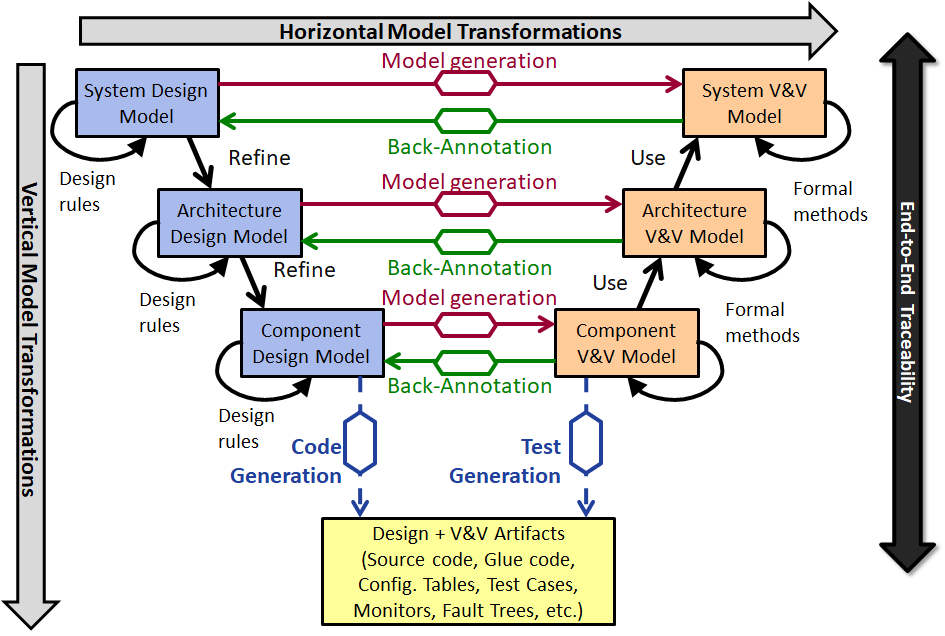
\includegraphics[width=.65\textwidth]{figures/mbse}
%\caption{Models transformations in model-based systems engineering}
%\label{fig:mbse}
%\end{figure}


Automated code generators (also called vertical MTs) improve productivity by synthesizing provenly correct source code of a safety-critical application from a validated model.% \cite{Sturmer-TSE2007}. 
In addition to source code generation, MBSE tools can synthesize other design artifacts (such as configuration tables, fault trees, test cases, documentation) and provide support for end-to-end traceability.% \cite{Aizenbud-IBMSystems-2006}. 
MBSE changes the traditional V-model of systems engineering into a Y-model where certain certification artifacts are synthesized automatically from models of proven quality used at different levels of abstraction.

%\subsection{Summary}
In Stage 1, my research was characterized by (1) proposing novel, foundational concepts, (2) developing innovative and scalable techniques, (3) architecting and maintaining cutting edge prototype tools based on solid foundations, (4) continuously benchmarking and empirically evaluating these tools, and (5) using these results at design time in a wide range of applications in tools used for engineering critical systems (like avionics and automotive). 

\subsection{Scalable incremental model queries: Techniques and tools}

\paragraph{Results.}
With my graduate students, G. Bergmann, M. Búr, Á. Hegedüs, Á. Horváth, G. Szárnyas, and I. Ráth, we developed highly scalable incremental techniques for continuously evaluating graph queries over large domain-specific instance models used in design and validation tools of critical systems. We turned scientific results \cite{models-2010-incquery,scp2015,models2014-iqd,icgt2015,sosym2016-viatra-invited} into mature scalable software tools, which instantly re-evaluate validation rules over domain-specific graph models with millions of elements. 

\paragraph{Impact.}
The \href{https://www.eclipse.org/viatra/}{VIATRA open source project} has been actively \emph{used at large companies and research institutes} (e.g. Thales, Airbus, Ericsson, ThyssenKruppPresta, Embraer, NASA JPL), and in \emph{industrial modeling tools} (e.g. Papyrus, Capella, Artop). It provides the basis of \emph{innovative products} (\href{https://incquerylabs.com/incquery/}{IncQuery for MagicDraw, IncQuery Server}) developed at IncQuery Labs Ltd. It has been \emph{regularly used a baseline in performance comparisons} by leading researchers (e.g. D. Kolovos, J. Cabot, H. Giese). I \emph{delivered several keynote talks} on related topics at major scientific conferences and summer schools. Related papers \cite{models-2010-incquery,icmt2011,ase2011-tool,ecmfa2011,models2014-iqd,scp2015,icgt2015,sosym2016-viatra-invited} have been cited over 400 times. 
% and \cite{models2018-tool} received a \textbf{Best Tool Paper Award} at the MoDELS 2018 conference. 

\paragraph{My role.}
All major contributors of the incremental graph query technology are my former PhD students. I have been the strategic leader of the research line until 2016 when the development of the open source framework was taken over by software engineers at IncQuery Labs Ltd, a high-tech company co-founded together with my former graduate students. This line of research has been funded by numerous national and international competitive research projects: I was the site leader at BME of \emph{collaborative European projects} (e.g. SENSORIA, SecureChange), and the principal investigator (PI) of an ERC Starting Grant application (CERTIMOT) which went to the final round, but became out of budget, and later it received partial funding from the Hungarian Research Agency (ERC-HU). 
%VIATRA technology received significant extra funding at IncQuery Labs, which is not detailed here. 


\subsection{Novel model transformations concepts}

\paragraph{Results.}
With my students, A. Balogh, Z. Balogh, G. Bergmann, Á. Hegedüs, Á. Horváth, I. Ráth, Z. Ujhelyi, we proposed novel model transformation concepts to capture mappings within and between various modeling languages. The scientific results provided foundations of the open source \href{https://www.eclipse.org/viatra/}{VIATRA} model transformation framework \cite{SCP2002,ASE2002,uml2004-meta,scp-2007,sosym2016-viatra-invited} which has been successfully developed along three generations since 2000. Novel concepts proposed by us for the first time include \emph{change-driven transformations} \cite{Rath-models09,sosym2011-cdt}, \emph{model transformation by example} (MTBE) \cite{models2006-varro,sosym2008-mtbe}, \emph{reactive transformations} \cite{icmt08-rbov08,icmt2015,sosym2016-viatra-invited} or \emph{model transformation slicing} \cite{ase2011-mtslice,icst2012}.

\paragraph{Impact.} 
In addition to its industrial use, we published our results on the VIATRA framework at major scientific venues of model-driven engineering including \cite{SCP2002,ASE2002,uml2004-meta,models2006-varro,scp-2007,Bergmann-icmt09,Rath-sosym09,Rath-models09,Bergmann-sttt10}, which have been cited well over 2000 times. The paper \cite{uml2004-meta} got the \textbf{10-year Most Influential Paper Award} at the IEEE/ACM MODELS 2014 conference (the main scientific forum of my research area), and I was invited to write an expert panel paper to the Software and Systems Modeling journal (SoSyM) \cite{sosym2016-viatra-invited}. Our first paper on change-driven transformations \cite{Rath-models09} received \textbf{Springer Best Paper Award} at IEEE/ACM MODELS 2009. The concepts of MTBE have been followed by 12 independent research groups worldwide. I delivered \emph{several keynote talks} at international conferences and summer schools on related topics.

\paragraph{My role.} 
The first open source version of VIATRA was developed by my graduate students, and I served as the strategic leader of the project until 2016 when development was taken over by IncQuery Labs Ltd. Therefore, I played key role in maturing a research prototype into an industrial framework. I was the main contributor (and hence, the first author) of the expert panel paper invited to the SoSyM journal.  I was the main supervisor of 5 PhD students and co-supervisor of 2 PhD students in addition to 20+ MSc students doing research and development on related topics. Co-founding IncQuery Labs enabled to keep together the core team for 15 years by now. I was the principal investigator (PI) of three IBM Faculty Awards, and an ERC-HU Starting Grant application and the site leader of various collaborative European projects (e.g. SENSORIA, SecureChange, MONDO) .

%My role in the related projects that funded this line of research is the same as in the previous line

\subsection{Performance benchmarks for model queries and transformations}
\paragraph{Results.}
Together with G. Varró and A. Schürr, we proposed the \emph{first performance benchmark for model transformation tools} in \cite{vlhcc05-vsv}. Since then, developing and maintaining performance benchmarks have been a focal topic of my research group. With my students, G. Bergmann, Á. Horváth, B. Izsó, G. Szárnyas, I. Ráth, Z. Ujhelyi, we systematically assessed the performance of various model query technologies \cite{Bergmann-sttt10,scp2015,ttc2015} of different modeling tools. 
%for different technological platforms along the Train Benchmark. 
In collaboration with researchers from University of Szeged, IncQuery was successfully used for detecting anti-patterns in source code of large projects \cite{csmr2014,ist2015}.

\paragraph{Impact.} 
Our first paper \cite{vlhcc05-vsv} triggered a series of annual Transformation Tool Contests (over 12 editions) and it received a \textbf{Most Influential Paper Award} at IEEE VL/HCC 2016. Moreover, \cite{csmr2014} received the \textbf{Best Paper Award} at CSMR-WCRE 2014. The Train Benchmark \cite{ttc2015} has been used by other researchers (e.g. D. Kolovos, X. De Carlos, G. Varró, G. Hinkel, H. Giese) for performance comparison from several independent research groups. Related papers have been cited over 275 times.

\paragraph{My role.} 
I was one of the three researchers who proposed the first benchmark for model transformations in 2005. 
%Benchmarking was a focal topic of my PhD student G. Szárnyas, while 
Later, I was a co-organizer of the first open transformation tool comparison as part of the AGTIVE 2007 conference \cite{agtive07-toolcontest}. My students (G. Bergmann, Á. Hegedüs, Á. Horváth, B. Izsó, I. Ráth, Z. Ujhelyi) made significant contributions to past benchmarking activities. I was the site leader at BME of the MONDO FP7 project, 
%and a collaborator in the MOGENTES FP7 project, 
which financed some of the related research activities.

\subsection{Rule-based guided design space exploration}

\paragraph{Results.}
Design space exploration (DSE) aims to derive design candidates fulfilling various design constraints from an initial design sketch by applying a pre-defined set of operations. We proposed the concept of \emph{rule-based guided design space exploration} \cite{Horvath-models09,sosym2011-csp,ase2011-dse,ause2015,ase2014,mpm2014} to incorporate complex structural consistency constraints frequently present in architecture models of automotive and avionics applications. The exploration process can be heuristically guided by hints obtained from the designer. DSE was applied to provide quick fixes in design environments built for business modeling \cite{vlhcc2011}. 

\paragraph{Impact.} 
Our paper \cite{ase2011-dse} at the IEEE ASE 2011 conference received an \textbf{ACM Distinguished Paper Award}. Other researchers (e.g. H. Vangheluwe, S. Zschaler and M. Wimmer) conducted research building on our results. Key papers \cite{Horvath-models09,vlhcc2011,sosym2011-csp,ase2011-dse,ause2015,ase2014} received over 150 citations in total. 
%The VIATRA-DSE open source software won \emph{two first prizes at the 9th Transformation Tool Contest} (TTC 2016). The prototype software was evaluated at NASA Jet Propulsion Lab for high-level mission planning.

\paragraph{My role.} 
DSE exploration served as a key research topic for three PhD students (Á. Horváth, Á. Hegedüs, A. Nagy) under my supervision, and I was last author in most of the key papers. Global search-based techniques were developed in collaboration with H. Sahraoui and H. Abdeen \cite{ase2014} during my period as a visiting professor at Université de Montréal in 2014. I was the site leader at BME of the DIANA EU project (which funded the initial investigations), and the PI of the CERTIMOT ERC-HU project and the research grant offered by Embraer (which funded subsequent investigations).

\subsection{Design techniques and tools for critical systems}

\paragraph{Results.} 
With my students, G. Bergmann, Á. Hegedüs, Á. Horváth, I. Ráth, Z. Ujhelyi, we developed novel techniques that can be used in design and verification tools used for safety-critical systems. \emph{Soft traceability links} \cite{models2012,sosym2016-trace} were developed within a collaborative project funded by Embraer (the large Brazilian airframer) to enable the seamless integration of models developed in different tools based on incremental model queries. 
We proposed a \emph{formal validation technique for domain-specific languages} \cite{models2013} in the same project to find inconsistencies in language specifications. The \href{https://github.com/viatra/massif/}{Massif} open source project interconnects of Matlab Simulink models and EMF-based modeling tools. 

\paragraph{Impact.} 
We published our results at top scientific venues of model driven engineering (e.g. MODELS conference, SoSyM journal). This line of research (started as part of the DIANA FP6 European project with large avionics companies) evolved into a 2-year \emph{collaborative industrial project funded by Embraer}, the large Brazilian aircraft manufacturer. As such, it had significant industrial impact. Our formal validation approach \cite{models2013} received \textbf{Springer Best Paper Award} at the IEEE/ACM MODELS 2013 conference. The Massif open source project has been used at several companies including Thales and MapleSoft.

\paragraph{My role.} 
I was the main supervisor of all the student contributors listed above, and consequently, I was the last author of most publications along this research line. I was the principal investigator of the collaborative project funded by Embraer, and I was the site leader at BME in the DIANA FP6 European project and the CONCERTO ARTEMIS project. I was a co-founder and Vice-President of Research and Development at OptXware Ltd., a start-up company founded at BME, which was partially acquired in 2013 by a large European company in the automotive domain. 
%An automotive design tool was developed at OptXware for a major tool vendor, which was a ke


\section{Recent Research Results: Stage 2 (2015- )}

\subsection{High-level overview of the research program}

\paragraph{Motivation.}
 A smart\& safe cyber-physical system (CPS) \autoref{fig:smart-safe-cps} is a software-intensive decentralized system that autonomously perceives its operational context and adapts to changes over an open, heterogeneous and distributed platform with a massive number of nodes, dynamically acquires available resources and aggregates services to make real-time decisions, and resiliently provides critical services in a trustworthy way. 
%Several challenges of such systems have been identified in \cite{Sztipanovits2012,Lee2014,Krupitzer2015,Cengarle2013,CPSoS2015}. 

In an open, interconnected and decentralized CPS, the components, the services, the underling execution platform and the environment may continuously evolve and change, thus distinction between design-time and run-time is blurred. %\cite{Baresi2010}. 
First, runtime information on services, platforms and deployment can be captured by runtime models %\cite{Blair2009,Szvetits2013} 
and operations on models will have direct effects on the running system. Then dynamic changes in requirements, services, resources, deployed configurations and reconfiguration rules need to be handled. Consequently, optimization and exploration will be pushed to runtime to guarantee that new deployment configurations do not jeopardize safety.

Recent advances in machine learning drives innovation in many sectors, e.g. to decrease energy consumption in smart buildings, to better adapt to current demands in smart factories or to prevent accidents in connected cars. But one needs to \emph{guarantee the trustworthiness of smart systems in a continuously evolving open environment}. It is a major challenge today for our society to prevent major future failures of such autonomous decentralized systems.

\begin{figure}
\centering
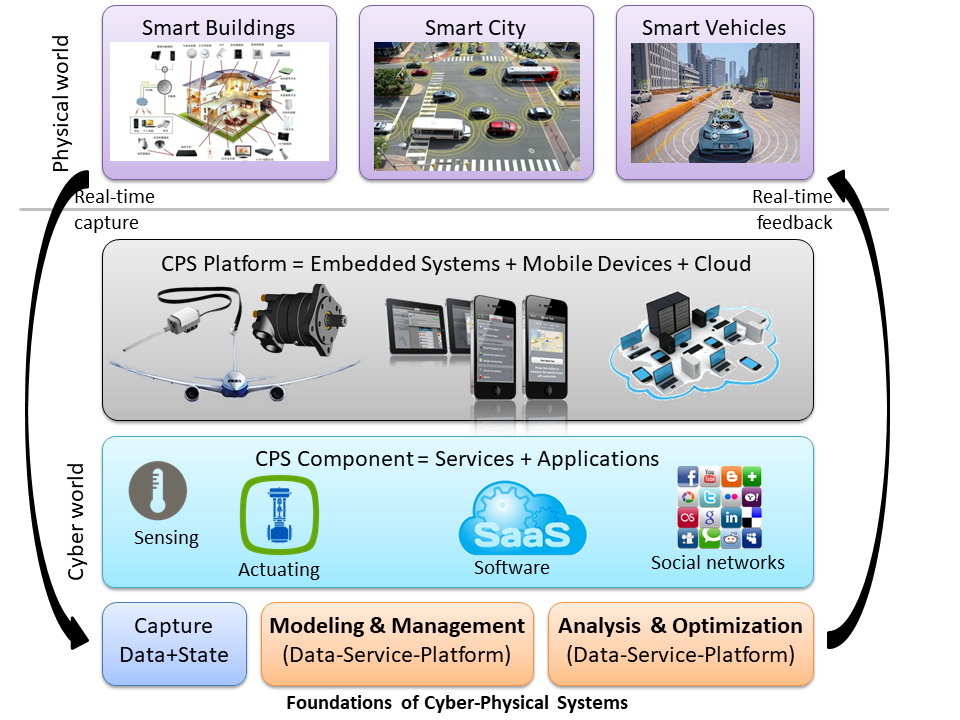
\includegraphics[width=.65\textwidth]{figures/smart-safe-cps}
\caption{Smart and safe cyber-physical systems}
\label{fig:smart-safe-cps}
\end{figure}


\paragraph{Objectives.}
My recent research has been aiming to develop innovative \emph{design, synthesis, management, validation and optimization techniques and tools}  for engineering smart and safe CPSs. In particular, my research group has been working to address two key long-term objectives:

\begin{itemize}
\item \textbf{Long-Term Objective 1}: How to \emph{design and manage} dynamically evolving smart\& safe CPSs to fulfill multi-domain requirements (e.g. consistency, extra-functional or physical)?
\item \textbf{Long-Term Objective 2}: How to \emph{guarantee or validate} that smart\& safe CPS with multi-domain requirements deliver quality of service in an open and changing environment?
\end{itemize}

%\paragraph{Research environment.}
%This research has been carried out in a rather unique and unconventional research environment. In 2015, I successfully acquired a Hungarian prestigious and highly selective Research Chair position funded by the Hungarian Academy of Sciences to run the \href{https://mta.hu/lendulet/az-mta-lendulet-kutatocsoport-halozata-105402}{MTA-BME Lendület Cyber-Physical Systems Research Group}. Here I was main supervisor of five PhD students, but I also provided co-supervision or strategic guidance for six other PhD students (partially affiliated to the project) who are supervised by young faculty members at the Department of Measurement and Information Systems. 
%In response to the increasing direct political influence on academic institutes and research funding imposed by the Orbán Government in Hungary, I joined the Department of Electrical and Computer Engineering at McGill University as a full professor in 2016. Since then, I have been coordinating research of a virtual (trans-Atlantic) group with frequent visits of Hungarian students at McGill.
%
%Furthermore, I was directly involved in strategically shaping proposals for European projects and training networks where IncQuery Labs Ltd was the involved partner.  Along these lines, we achieved the following major results in the past 5-6 years. 

\subsection{Distributed graph queries for runtime monitoring} 

\begin{table}[htb]
\footnotesize
\begin{tabular}{@{}p{5cm}p{11cm}@{}}
\toprule
%\textbf{ECSE 429 Questions} & \textbf{F18} \\ 
%\toprule
Publications &  \cite{sttt-2019-cps,fase2018-cps,wf-iot-2019,models2019-wcet} (all refereed), 1x \textbf{Best Paper Award} 
\cite{fase2018-cps} \\ \midrule
Graduate students at McGill & M. Búr, F. Khan \\ %\midrule
McGill undergraduates (SURE) &  C. Grosdidier \\ \midrule
%Past graduate students &  I. Ráth, Á. Horváth \\ \midrule
MTA-BME Lendület collaborators & A. Vörös \\ \midrule
%Other collaborators & G. Szilágyi, Z. Micskei, L. Balogh, B. Hegyi, B. Horváth, Z. Mázló \\ \midrule
%Key impact &  Publications at leading venues (including ICSE),  \\ \midrule
Funding &  NSERC DG (CA), MTA-BME Lendület (HU), NSERC Engage (under review) \\ %\midrule
\bottomrule
\end{tabular}
\caption{Summary: Distributed graph queries for runtime monitoring}
\end{table}

\paragraph{Motivation.} 
Since upfront formal verification is typically infeasible for smart CPSs, runtime monitoring is a common practice to continuously detect the violation of (safety) properties at runtime. Runtime monitoring has been addressed by runtime verification (RV) techniques %\cite{Leucker2009,Mitsch2014} 
which provide formal precision, but offer a low-level specification language (with simple atomic predicates to capture information about the system). 
%Recent RV approaches \cite{Havelund2015} started to exploit rule-based techniques over a richer (relational or graph-based) information model. 
Runtime models %\cite{BlairBF09,Szvetits2013} 
provide a rich knowledge representation to capture the runtime operational state and context of a smart CPS as typed and attributed graphs to serve as a unifying semantic basis for runtime assurance of self-adaptive systems (SAS).
%in \cite{Cheng2014,Vogel2014}. 
While graph models are widely used internally in various design tools for CPS (e.g. Capella, Artop), real-time CPSs dominantly use low-level data structures with static (i.e. compile-time) memory allocation to ensure resource constraints such as memory limits or deadlines, which is a major limitation.
% Unfortunately, \emph{such static data models are unable to capture dynamically evolving contextual information where there is no a priori upper bound on relevant contextual objects} (e.g. many pedestrians may be in contextual range of a self-driving car), which is a major limitation. 

\paragraph{Results.}
Together with my M. Búr (my PhD student at McGill), G. Szilágyi and A. Vörös, we proposed different graph-based technologies for runtime monitoring purposes in smart\& safe CPS, showcased in the context of the MoDeS3 research demonstrator \cite{nfm2018}. For that purpose, we adapted existing model management and distributed graph query techniques to be deployed over a heterogeneous, decentralized execution platform with resource constraints \cite{fase2018-cps}.  Since graph queries have traditionally been used at design-time by executing them on desktop computers (or servers), their adaptation to a resource-constrained runtime platforms is a highly complex challenge. 
We evaluated the performance of our graph query based runtime monitors \cite{wf-iot-2019} over the DDS (Data Distribution Service) platform, which is a standard of the Object Management Group (OMG). Furthermore, in a very recent journal paper \cite{sttt-2019-cps}, we precisely formalized the behavior of our distributed algorithms and carried out a more extensive scalability evaluation. 
In order to use such graph query techniques for monitoring purposes in hard real-time applications, the worst case execution time (WCET) of the monitoring programs needs to be estimated. Thus in our recent MODELS 2019 paper \cite{models2019-wcet}, we proposed a long-term research agenda and an initial approach that exploits existing WCET analysis tools for calculating WCET for graph queries.

\paragraph{Impact.} 
We published several papers at leading conferences  \cite{fase2018-cps,models2019-wcet} and journals \cite{sttt-2019-cps}. Our paper \cite{fase2018-cps} received an \textbf{EASST Best Paper Award} at ETAPS 2018 (1 award out of over 140 papers). The MoDeS3 framework has been demonstrated at numerous industrial and other public events at BME (e.g. at the annual Researchers Night). These conceptual results have been successfully used in the MoDeS3 open demonstrator for smart and safe CPSs \cite{nfm2018}. I delivered a keynote talk at Ericsson Industrial Day 2016, at the CSCS 2016 Hungarian conference for PhD students, and several invited lectures at the DSM-TP international summer school in several consecutive years. Our results will provide a basis for an upcoming industrial collaboration with Predikat Inc. (Canada) where runtime monitoring of performance degradations in multi-tier web applications will be carried out (the NSERC Engage project is still under review).
% and in an initial prototype developed for the successful Hungarian start-up TeqBall.

\paragraph{My role.}
I was the strategic initiator of this line of research. I was also the main supervisor of M. Búr (PhD student at McGill) and provided strategic guidance for A. Vörös (assistant professor at BME). I contributed to the precise mathematical formulation of the results \cite{fase2018-cps,sttt-2019-cps,models2019-wcet} and also to the textual contents of all publications. I was the PI of a related NSERC Discovery Grant (Canada), an NSERC Engage application and the Lendület Research Group (Hungary). 

\subsection{Automated generation of domain-specific graph models: The CORE-DISC challenge}

\begin{table}[htb]
\footnotesize
\begin{tabular}{@{}p{5cm}p{11cm}@{}}
\toprule
%\textbf{ECSE 429 Questions} & \textbf{F18} \\ 
%\toprule
Publications &  \cite{fmhe2018,sosym2017-dsl,sttt-2019-div,fase2018-diverse,fase2016-solver,icse2018-solver,icse2019-tool,MODELS2016-metrics,MODELS2016-bx,models2018} (all refereed), 2x defended PhD theses (by O. Semeráth, G. Szárnyas) \\ \midrule
Graduate students at McGill & A. Babikian \\ %\midrule
Graduate research trainees at McGill &  O. Semeráth, G. Szárnyas (PhD students defended at BME, supervisor), K. Marussy (PhD student at BME, co-supervisor)  \\ %\midrule
McGill undergraduates (SURE) &  A. Babikian, S. Pilarski, A. Li, B. Chen, L. Li, M. Ding, V. Gidla \\ \midrule
Past graduate students &  G. Bergmann, Á. Horváth \\ \midrule
MTA-BME Lendület collaborators & R. Farkas, A. Vörös \\ \midrule
Other collaborators & Z. Szatmári \\ \midrule
%Key impact &  Publications at leading venues (including ICSE),  \\ \midrule
Funding &  NSERC DG (CA), MTA-BME Lendület (HU) \\ %\midrule
\bottomrule
\end{tabular}
\caption{Summary: Automated generation of domain-specific graph models}
\end{table}

\paragraph{Motivation.}
Graphs are key abstractions in science and engineering. They may represent linked data in graph databases, complex designs of cyber-physical systems or critical contextual situations for autonomous systems. Synthetic graph generators are essential when the use of real graph models is restricted (to respect privacy regulations or intellectual properties of companies) or impractical (to find corner-cases for safety assurance). I initiated the CORE-DISC \emph{long-term research program program} \cite{fmhe2018} to develop a next generation of synthetic graph generator techniques and tools that are customizable to different application domains to derive graph models which are simultaneously \emph{CO: consistent} (graphs shall satisfy various structural logic constraints of the domain), \emph{RE: realistic} (synthetic graphs shall resemble real graphs of a given domain), \emph{DI: diverse} (any pair of graphs shall be structurally distant from each other) and \emph{SC: scalable} (the graph generator shall be able to derive large graph models). Such synthetic graphs are intended to be used as test cases in tool qualification process prescribed by safety standards.% (like DO-330).

\paragraph{Results.} 
As consistency appeared to be the most difficult property to achieve, our initial investigations \cite{fase2016-solver,sosym2017-dsl} aimed to derive consistent graph models with the use of existing logic solvers like Alloy with Kodkod (from MIT) 
%\cite{Torlak2007} 
or Z3 (from Microsoft Research) %\cite{Moura-tacas2008}, 
but none of these attempts were able to scale by failing generate models with over 100 graph nodes. Therefore, we developed a novel \emph{consistent graph solver} \cite{icse2018-solver,icse2019-tool}(with my students, O. Semeráth, A. Nagy, G. Szárnyas, A. Babikian and S. Pilarski) for automatically generating consistent graph models by implementing a novel refinement calculus over partial models \cite{fmhe2018} and using an approximation technique based on constraint rewriting \cite{icmt2017}. Our consistent graph solver \cite{icse2018-solver,icse2019-tool} scales 1-2 orders of magnitude better than competitors that use background logic solvers and its scalability is comparable to search-based techniques %\cite{Soltana2017} 
while uniquely providing both consistency and completeness guarantees. We successfully applied the model generator for incremental backward propagation of view models \cite{MODELS2016-bx} as well as for incremental view model synchronization \cite{models2018}.

Moreover, we provided the first characterization of \emph{realistic models} in \cite{MODELS2016-metrics,fmhe2018} by adapting various graph metrics from network science and evaluating them on graph models taken from six different domains of software and systems engineering. By adapting graph shapes, %\cite{Rensink}, 
we proposed various \emph{model diversity metrics} \cite{fase2018-diverse,sttt-2019-div} by which generalize and subsumes several existing coverage metrics used for testing of model transformations. We extended our model generator and showed that it derives more diverse models than its direct competitors \cite{fase2018-diverse,fmhe2018,sttt-2019-div}. 

%aimed  Generating consistent After a series of initial results , we rea attempts with negative scalabil results 

\paragraph{Impact.}
We published our results in a series of papers at leading conferences and journals of software engineering including 1 book chapter, 1 journal paper at SoSyM \cite{sosym2017-dsl}, 1 at \cite{sttt-2019-div} in Software Tools on Technology Transfer (Springer), 2 papers at MODELS \cite{MODELS2016-bx,models2018}, 2 papers at FASE \cite{fase2016-solver,fase2018-diverse}. I also two invited talks on this topic: one at the CSER 2017 conference in Montreal and one at the Search Based Model Engineering Workshop at King's College London in 2018.
As a special highlight, we published a research paper \cite{icse2018-solver} and a tool paper \cite{icse2019-tool} at ICSE, the prime general-purpose software engineering conference, which is a major success as no modeling papers had been published in the previous three editions of ICSE. 
The news about our ICSE paper \cite{icse2018-solver} was \emph{featured on the front page of the Hungarian Academy of Sciences} (\href{http://mta.hu/english/innovation-of-hungarian-researchers-could-revolutionise-car-industry-design-technology-testing-108434}{Eng}, \href{http://mta.hu/tudomany_hirei/magyar-kutatok-eredmenye-forradalmasithatja-az-autoipari-tervezoeszkozok-teszteleset-108355}{Hun}) and shared by \emph{six major news portals in Hungary}, and I received three invitations for interviews in radio channels. 
%Our approach (published in \cite{sosym2017-dsl,act2017,fmhe2018,fase2018-diverse,icse2018-solver,icse2019-tool}) \emph{scales 1-2 orders of magnitude better} than competitors using state-of-the-art logic solvers like Alloy (MIT) or Z3 (Microsoft Research) and its scalability is comparable to search-based techniques \cite{Soltana2017}. 

%The model generator tool \cite{icse2018,icse2019-tool} provides 1-2 orders of magnitude better scalability compared to exis
%Already the initial results for the formal validation technique for DSLs \cite{models2013} (extended later to the journal paper \cite{sosym2017-dsl}) received Best Paper Award at the IEEE/ACM MODELS 2013. 

\paragraph{My role.}
I was the sole PhD supervisor of key contributors (O. Semeráth, G. Szárnyas, A. Nagy) and MEng students (A. Babikian, S. Pilarski) of this research line, hence being the last author in all papers above. I was the first author of \cite{fmhe2018}, which presents a long-term research agenda and challenges for automated graph model generation. My technical contributions  include some precise foundations and key theorems for the refinement calculus over partial models. I was the PI of the Lendület project and NSERC Discovery Grant that provided funding for the involved students.


\subsection{Secure collaborative modeling}

\begin{table}[htb]
\footnotesize
\begin{tabular}{@{}p{5cm}p{11cm}@{}}
\toprule
%\textbf{ECSE 429 Questions} & \textbf{F18} \\ 
%\toprule
Publications &  \cite{sosym2017-mondo,ieeesw2018,MODELS2016-access,fase2016-merge,esec-fse2017,%
models2017,vlhcc2018,commitmde2016,commitmde2017} (all refereed), 1x PhD thesis (under review), 
1x \textbf{Distinguished Paper Award} \cite{MODELS2016-access}
\\ \midrule
Graduate students at McGill & M. Búr  \\ %\midrule
Graduate research trainees at McGill &  C. Debreceni (PhD student at BME, main supervisor) \\ \midrule
Past graduate students &  G. Bergmann, I. Ráth \\ \midrule
Other collaborators &   De Carlos, X. Mendialdua and S. Trujillo (Ikerlan, Spain), A. Barisic, V. Amaral, M. Goulao (Nova Univ. Lisbon, Portugal) \\ \midrule
Funding &  MTA-BME Lendület (HU), MONDO (EU), NSERC DG (CA), %Bolyai scholarship (HU, secured by G. Bergmann)
 \\ %\midrule
\bottomrule
\end{tabular}
\caption{Summary: Secure collaborative modeling}
\end{table}

\paragraph{Motivation.}
As a common industrial practice in model-based systems engineering, system integrators frequently outsource the development of various components to subcontractors in an architecture-driven supply chain where the collaboration between cross-organizational teams is facilitated by sharing models stored in model repositories. However, effective cross-organizational collaboration is hindered by numerous factors, such as (1) lack of appropriate fine-grained access control management to protect the intellectual property rights (IPR) of involved parties, (2) model fragmentation, or (3) the inability to combine online (GoogleDoc type) and offline (Git or SVN-like) collaboration schemes. 

\paragraph{Results.} 
Together with C. Debreceni, M. Búr, G. Bergmann and I. Ráth, we developed a collaborative modeling framework \cite{esec-fse2017,ieeesw2018} that enhances modeling repositories by providing secure views as an extra protection layer with rule-based high-level access control simultaneously enforced for both offline and online collaboration scenarios and adapted to software configuration management. As a novel underlying concept, we developed a rule-based fine-grained access control technique using bidirectional transformations \cite{MODELS2016-access}. The soundness of the core collaboration scheme was formally proved and successfully applied for both online and offline collaborations in \cite{sosym2017-mondo}. 
Further technical details about the fine-grained model-level access control were published in two peer-reviewed workshop papers \cite{commitmde2016,commitmde2017}. 
To enhance the practical usefulness of the collaborative modeling framework, we developed an automated model merge technique driven by design space exploration \cite{fase2016-merge} (which was evaluated in a collaborative user study \cite{vlhcc2018}). Furthermore, we successfully developed an approach \cite{models2017} to implement the concepts of property-based locking that prevents unintentional model modifications during extensive collaboration. 

\paragraph{Impact.} 
We published seven research papers \cite{fase2016-merge,MODELS2016-access,models2017,esec-fse2017,vlhcc2018,sosym2017-mondo,ieeesw2018} at leading scientific forums (including conferences like MODELS, FASE, ESEC/FSE, VL/HCC and journals like Software and Systems Modeling and IEEE Software). Paper \cite{MODELS2016-access} received \textbf{ACM Distinguished Paper Award} at the MODELS 2016 conference, while the papers above received over 40 citations (Google Scholar). Related concepts were integrated into an innovative product developed by IncQuery Labs Ltd. \cite{models2018-tool}.
%Paper \cite{vlhcc2018} carried out a user study in an industrial setting as part of the MPM4CPS EU COST Action.

\paragraph{My role.} 
I was the strategic initiator of this research line, thus the last author in most related publications (except for the collaborative paper \cite{vlhcc2018}). I am the main supervisor of C. Debreceni and M. Búr who were major technical contributors of the framework. C. Debreceni has already submitted his PhD thesis, and his public defense is expected in Fall 2019. I was the site leader of the MONDO FP7 project at BME where this line of research was started, and the PI of the Lendület project which provided continuity. I helped G. Bergmann (who is an assistant professor at BME) to successfully apply to the prestigious János Bolyai Scholarship in Hungary in a related research topic. 

\subsection{Digital Multidisciplinary Analysis and Design Optimization Platform}

\begin{table}[htb]
\footnotesize
\begin{tabular}{@{}p{5cm}p{11cm}@{}}
\toprule
%\textbf{ECSE 429 Questions} & \textbf{F18} \\ 
%\toprule
Publications &  \cite{mdeintelligence2019} (refereed), 3x MEng thesis (in preparation) \\ \midrule
Graduate students at McGill & M. Rangappa, J. Dhaliwal \\ \midrule
Other collaborators &  M. Staniszewski, Frederic Villeneuve (and other Siemens engineers) \\ \midrule
Funding &  NSERC CRD with Siemens (CA) \\ %\midrule
\bottomrule
\end{tabular}
\caption{Summary: Digital multidisciplinary analysis and design optimization platform}
\end{table}

\paragraph{Context.}
Gas turbines are a commonly used type of internal combustion engine used for power generation. The development of gas turbines requires creation of many different linked models by mechanical engineers. These models are used in gauging performance, designing secondary air systems, combustion, and other subsystems. Creation of design models can span across dozens of design tools which can integrate many data formats, disciplines, and requirements, which introduces significant software engineering challenges. For example, the large number of models inherently results in a huge design exploration space during the development process of an entire engine. Furthermore, the actual tool workflows need to be seamlessly integrated with the underlying development processes.

\paragraph{Results.}
This industrial CRD project started in 2018, and we work on innovative software-as-a-service solutions to integrate various design, analysis and optimization tools driven by workflows. This line of research is carried out together with my McGill MEng students, Maruthi Rangappa, Jasvir Dhaliwal and Sebastian Pilarski, and in collaboration with leading Siemens managers (M. Staniszewski and F. Villeneuve). We aim to develop a cloud-based solution to systematically store and query simulation results to allow fast iterations and a more agile design process. Moreover, we aim to exploit advance machine learning techniques to bring expertise gained from field data and simulated data directly to the mechanical engineers working on engine design. Initial results and a research roadmap has been proposed in \cite{mdeintelligence2019}, while two MEng theses about a graphical workflow editor and an "analysis tool as a service" infrastructure are planned to be submitted by J. Dhaliwal and M. Rangappa in Fall 2019.

\paragraph{Impact.}
While the project is still in an early phase, we made significant technological impact within Siemens. A software prototype developed by Sebastian Pilarski's will serve as the baseline software architecture for a cloud-based simulation environment being developed at Siemens. We also published a joint vision paper with leading Siemens managers at a MODELS 2019 workshop \cite{mdeintelligence2019}. 

\paragraph{My role.}
I am a co-PI of the NSERC project (PI: M. Kokkolaras - McGill, co-PI: H. Moustapha - ETS), and the only software engineering professor in the collaboration. I was contributing to the entire project preparation and proposal writing phase. I am the main supervisor of the three MEng students working on the project. In 2018, I was an invited speaker at the Siemens Industrial Day at ETS (Montreal), and also gave a talk about the project for graduate students.


\subsection{Continuation of previous research lines}
\paragraph{Results.} 
Naturally, I also continued previous research lines started in Stage 1 of my career. Below I summarize and report results where major progress has been made after I joined McGill University. 

\begin{itemize}[leftmargin=0.5cm]
\item
\textbf{Benchmarks for incremental graph queries:}
With key contributions from G. Szárnyas (my PhD student), we prepared a journal paper \cite{sosym2017-tb} to extend the Train Benchmark with a cross-technology comparison of graph query techniques with over 10 tools (including relational databases, graph databases, Eclipse-based modeling tools, rule-based expert systems, etc.). Thanks to the free availability of its source code repository, the Train Benchmark has been actively used by four independent research groups within the model-driven engineering community.


\item 
\textbf{Model transformation techniques:}
Together with O. Semeráth, C. Debreceni (my PhD students), K. Marussy (co-supervised by me) and Á. Horváth, we published two papers at the MODELS conference about the incremental backward synchronization of model transformations \cite{MODELS2016-bx} and fully incremental view model transformations \cite{models2018}. 

\item
\textbf{Design space exploration:}
Thanks to the key contributions from my PhD students, A. Nagy and O. Semeráth, the VIATRA-DSE open source software won \emph{two first prizes at the 9th Transformation Tool Contest} (\href{https://www.transformation-tool-contest.eu/2016/solutions_cra.html}{TTC 2016}). Subsequently, the prototype software was evaluated at NASA Jet Propulsion Lab for high-level mission planning.

\item
\textbf{Formal verification of reactive systems:}
With V. Molnár, Á. Hajdu (graduate research trainees at McGill), B. Graics, A. Vörös, Z. Micskei, I. Majzik (staff members at BME and main supervisors of PhD student), we developed a high-level modeling language for semantically precise composition of reactive components defined by statecharts where each component may follow a different execution semantics (e.g. synchronous vs. asynchronous). The Gamma tool was demonstrated at ICSE 2018 \cite{icse2018-gamma} and the related research paper \cite{sosym-2019-gamma} is under review. I gave an invited talk and a tutorial about this line of research at the DSM-TP 2017 international summer school.


\end{itemize}


\subsection{International research collaborations}

While as a senior researcher, my main mission is to supervise graduate students and help them mature as independent researchers, I still continue participating in international collaborations that typically result in joint publications. Below I summarize a few joint initiatives from the past 3-4 years. 

\begin{itemize}[leftmargin=0.5cm]
\item \textbf{Server-side incremental queries } 
I actively collaborated with researchers and software engineers of IncQuery Labs Ltd. from the inception phase to develop an innovative, server-side product called IncQueryServer for TeamWork Cloud. The product exploits advanced graph query techniques to provide cloud-based server-side validation services over large system models captured in the standard SysML language. The product is  provided as an add-on to a popular cloud-based model repository product of NoMagic/Dassault Systems. We published a joint tool demonstration paper \cite{models2018-tool}, which  received a \textbf{Best Tool Paper Award} at the MODELS 2018 conference.

\item \textbf{Survey on model transformations} In 2017, I was invited to collaborate on a new survey assessing the state of the art of model transformation tools with N. Kahani, M. Bagherzadeh, J. Cordy and J. Dingel (all from Queen's University). The collaboration resulted in a joint paper \cite{sosym2019-mt} published at the SoSyM journal in 2019 and it already received 10+ independent citations.

\item \textbf{Complex event processing for runtime models}
As a continuation of past research \cite{models2014-stream} carried out with I. Dávid (Univ. Antwerp, Belgium) and I. Ráth to adapt the concepts of complex event processing for runtime models for stream processing, we published an extended journal version of our results which contained precise formalization of our concepts \cite{sosym2018-cep}. Certain concepts along this line were used in a proof-of-concept prototype developed for the successful Hungarian start-up TeqBall.

\item \textbf{User study on model merge techniques} 
Together with A. Barisic, V. Amaral, M. Goulao (researchers at Nova Univ. Lisbon, Portugal) and my PhD student C. Debreceni, we collaboratively carried out and published a user study \cite{vlhcc2018} to assess the usability of a novel model merge technique. In fact, the model merge technique \cite{fase2016-merge} was also a result of collaborative research within the MONDO project with X. De Carlos, X. Mendialdua and S. Trujillo (from Ikerlan, Spain). The execution of user study was mainly driven by the collaborators from Portugal (and partially supported by MPM4CPS EU COST Action), while we provided technical support for the focal tool of the user study. 
\end{itemize}


\section{Future Research}

%\subsection{Context}

\paragraph{Motivation.} 
Digitalization is a dominating trend in engineering in initiatives like Industry 4.0 or Internet-of-Things. The concept of \emph{digital twins} (i.e. digital replica of physical assets, processes, people, places, systems) requires developing and continuously maintaining a digital representation of design documents in the form of models using a multitude of design, validation and optimization tools. The traditionally separate design and operation phases are blurred by systematically recording operational (field) data and processing it by machine learning and software engineering techniques to provide useful input for next design cycles. Decision making in autonomous CPSs (like self-driving cars, or drones) relies upon runtime models collected by a network of sensors, and fused by various artificial intelligence techniques. 

\paragraph{Main challenge.}
While innovation for digitalization is driven by software and intelligent data processing techniques; however, there is too much optimism for their fast penetration to critical CPSs (like cars, aircrafts, space) while appropriate means of quality assurance is severely lacking, especially in the presence of an increased level of automation or autonomous behavior.
 
%\begin{itemize}
%\item[(1)] 
While dozens of software tools are necessitated to a fully digital design of a complex CPS, quality assurance for tools and integrated tool chains is insufficient and represents a major risk for digitalization. How to trust a digital twin if one cannot trust the software tool used for designing it? Software safety standards of critical avionics systems (\href{https://standards.globalspec.com/std/1461615/rtca-do-330}{DO-330}) prescribe that only the output of a qualified tool can be trusted, and such a tool should meet the same requirements as the critical system component it designs. However, it makes tool qualification extremely costly.

%\item[(2)]
Due to recent fatal accidents, the safety assurance of autonomous cyber-physical systems (like self-driving cars or autonomous drones) is still its infancy. Unfortunately, decades of verification and validation (V\&V) practices developed for traditional safety-critical software systems are not applicable to autonomous systems. Existing practices rely up exhaustive simulation for system validation, but statistical techniques do not provide sufficient level of dependability and coverage in case of extremely rare events where one combination of rare events may jeopardize safety.
%\end{itemize}

\paragraph{Objectives.}
As a high-level objective, my ongoing and future research aims to increase the level of trust in digitalization for CPSs by developing systematic validation techniques for design tool chains and autonomous systems by automatically synthesizing potentially unsafe or problematic corner-cases and contextual situations. While the potential of digitalization is unquestionable, this project will mitigate its risks and negative impacts.

In particular, I am interested in novel scientific foundations and scalable software tools for 
\begin{enumerate}
\item the integration and testing of design tools used in digitalization for CPS, 
\item the system-level assurance of autonomous CPS,
\item the systematic testing for intelligent CPS driven by machine learning. 
\end{enumerate}

\paragraph{System-level assurance of autonomous CPS}
%\paragraph{Key ideas.}
Since safety-critical autonomous vehicles need to interact with an immensely complex and continuously changing environment, their assurance is a major challenge, and upfront design time assurance is generally regarded to be practically infeasible. While systems engineering practice necessitates assurance on multiple levels,  existing research focuses dominantly on component-level assurance while neglecting complex system-level traffic scenarios.
Our research aims to address the system-level testing of the situation-dependent behavior of autonomous vehicles by combining various model-based techniques on different levels of abstraction. Major initial progress and a research roadmap (developed in a SURE project in Summer 2018 and later in collaboration with researchers from BME but still under my scientific leadership) is reported in a vision paper \cite{models2019-systest} accepted at the MODELS 2019 conference.

%(1) Safety properties are continuously monitored in challenging test scenarios (obtained in simulators or field tests) using graph query and complex event processing techniques.  (2) To precisely quantify the coverage of an existing test suite with respect regulations of safety standards, we provide qualitative abstractions of causal, temporal, or geospatial data recorded in individual runs into situation graphs, which allows to systematically measure system-level situation coverage (on an abstract level) wrt. safety concepts captured by domain experts.  (3) Moreover, we can systematically derive new challenging (abstract) situations which justifiably lead to runtime behavior which has not been tested so far by adapting consistent graph generation techniques, thus increasing situation coverage. (4) Finally, such abstract test cases are concretized so that they can be investigated in a real or simulated context.

%\begin{enumerate}
%\item Safety properties are continuously monitored in challenging test scenarios 
%(obtained in simulators or field tests) using graph query and complex event processing techniques.  
%\item To precisely quantify the coverage of an existing test suite with respect regulations of safety standards, we provide qualitative abstractions of causal, temporal, or geospatial data recorded in individual runs into situation graphs, which allows to systematically measure system-level situation coverage (on an abstract level) wrt. safety concepts captured by domain experts. 
%\item Moreover, we can systematically derive new challenging (abstract) situations which justifiably lead to runtime behavior which has not been tested so far by adapting consistent graph generation techniques, thus increasing situation 
%coverage. 
%\item Finally, such abstract test cases are concretized so that they can be investigated in a real or simulated 
%context.
%\end{enumerate}

%\subsection{Testing of data sets used for machine learning in CPS design}
%
%\paragraph{Objectives.} Even when a large amount of field data is available as a training set, machine learning techniques provide no guarantees that this training set covers particular corner cases and rare events. We plan to devise an iterative and incremental approach which continuously evaluates a training set with respect to some coverage criteria over an abstract (graph-level) equivalence class, and then uses a graph generator (see below) to systematically derive test data for uncovered partitions of training data.
%
%\subsection{Auto-generation of consistent, realistic, diverse and scalable models}
%\paragraph{Objectives.} As a cross-domain underlying research line, we aim to develop automated synthetic graph generators with precise foundations, efficient algorithms and open-source scalable software prototype implementation to derive domain-specific graph models which are \emph{simultaneously consistent, realistic, diverse and scalable}. 
%Since graphs provide key abstractions of complex information in science and technology (including  design and runtime information of complex, software-intensive CPS), auto-generated graph models can serve as test cases or benchmarking purposes, especially, in data intensive, decentralized applications.

\section{Research Funding}

\subsection{Past research funding (Stage 1)}
In the first stage of my career, I was successful in attracting a variety of substantial research funding with both individual and collaborative research projects, with academic as well as industrial funding. 

\paragraph{Collaborative European projects: }
Since 2005, I was the site leader or research coordinator at BME for a series of collaborative European projects. The \emph{SENSORIA project} (2005-2010) aimed to provide precise software engineering techniques for next-generation service-oriented overlay computers. The \emph{DIANA project} (2006-2010) involved large avionics companies to provide a distributed and equipment-independent environment for avionics applications compliant with the ARINC 653 standard. The E-Freight project (2010-2013) aimed to improve on European e-freight capabilities for combined transport routes. The SecureChange project (2009-2012) developed various security engineering techniques used for evolving software-intensive systems. Finally, the MONDO project (2013-2016) was concerned with the development of scalable modeling and model management techniques deployed over a cloud platform.
I was involved in these projects starting both during the proposal writing as well as the actual execution phase. I was the scientific leader for different work packages, coordinated the development of project demonstrators, and altogether, I successfully collaborated with well over 100 researchers in Europe.

\paragraph{Individual research grant applications: }
I was also successful in grant applications where I was the sole PI. In particular, my ERC Starting Grant project (CERTIMOT: Design and Analysis Techniques for Certifiable Model Transformations) went to the final round of reviews at the European Commission with a supportive score of 7/8, but it became out of budget. Finally, it received partial funding from the Hungarian Research Agency and ran between 2010 and 2014. My application to the MTA Lendület research chair program is detailed below.


\paragraph{Industrial funding: }
I was the principal investigator of a two-year research project (TRANS-IMA) funded by Embraer, the large Brazilian airframer to develop innovative model-based avionic tools for their systems engineering process (total funding: 200,000 EUR). Previously, I was the three times recipient of the IBM Faculty Award offered by IBM TJ Watson Research Center (total amount of 36,000 USD). I was research coordinator for two collaborative projects with Nokia Research Centre (Budapest) on high-availability service platforms and model-driven development techniques (approx. 40,000 EUR).

\subsection{Recent research funding (Stage 2)}
Since 2015, I successfully continued to secure substantial amount of research funding with a total amount of Canadian funding over 1.46 million CAD as PI or co-PI (own share of funding: 580,000 CAD), and additional own funding over 160 million HUF (equivalent of over 730,000 CAD) in Hungary. Except for my start-up grant offered by McGill University, all other grants were secured on a competitive basis. Further financial details of funding are listed in my CV.

\paragraph{NSERC CRD: Digital Multidisciplinary Analysis and Design Optimization Platform (2018-2023): }
We started a 5-year long multidisciplinary collaborative research and development (CRD) project co-funded by Siemens Canada and NSERC targeting a design platform for designing aeroderivative gas turbines. The total funding of the project is around 1.2 million CAD (with roughly 25\% is reserved to my own research). 

%Furthermore, I gave two invited talks at the Siemens-ETS Industry 4.0 Day in Montreal in 2018. 

\paragraph{NSERC Engage (2019-2020): Automated identification of performance regressions in a multi-tier web applications, under review}
With its innovative Predicate AIOps tool suite, our industrial partner, Predikat Inc. offers innovative solutions to prevent down-time and predict traffic for multi-tier web applications for companies providing business-critical
Software-as-a-Service solutions deployed over virtual machines or as microservices using a complex,
multi-layered software stack composed of heterogeneous technologies. As a specific problem at Predikat,
finding the root cause of identified performance regressions is a time-consuming manual task. This project
aims to identify performance bottlenecks in multi-tier web applications by runtime monitoring and then provide
automated root cause analysis to trace the bottleneck to the relevant component in real-time, thus removing the
burden of manual troubleshooting from DevOps engineers. As such, it would further enhance the existing
capabilities of the Predicate AIOps tool suite. The project is under evaluation, and it is expected to run for six months starting in Fall 2019.

\paragraph{NSERC Discovery Grant (2016-2021): Model-based Design and Validation Techniques for Smart and Safe
Cyber-Physical Systems:}
Due to its flexible nature, my NSERC Discovery Grant provided funding for students without having an industrial project. This included Márton Búr (PhD student at McGill), and Faizan Khan (MEng student at McGill) to carry out research in the context of Internet-of-Things applications of cyber-physical systems. In addition, it funded a total of 9 undergraduate students who participated in early research activities as part of the Summer Undergraduate Research in Engineering (SURE) program. Furthermore, travel costs of several Hungarian PhD students who visited my as McGill graduate research trainees were covered.

\paragraph{LiveIDE: Live Integrated Development Environment for Software-Intensive Communication Systems (2017): }
In 2017, I led the submission of a proposal as principal investigator for a three-year NSERC Strategic Partnership Grant for Projects with G. Mussbacher, J. Kienzle (McGill), H. Sahraoui and E. Syriani (UdeM) as co-PIs and Ericsson Montreal as supporting industrial partner. NSERC offered to accept the project without further changes as a collaborative research and development (CRD) project due to its industrial relevance, but unfortunately, this CRD contract was not signed as the main contact and project lead at Ericsson left the company (after 20 years).

\paragraph{MTA-BME Lendület Cyber-Physical Systems Research Group (2015-2020)}
This prestigious and highly selective research chair program is run by the Hungarian Academy of Sciences, and each year a total of 12-15 researchers below the age of 45 are awarded nation-wide. In 2015, I was only the third ever recipient in the field of computer science. The project provided partial funding for 10 PhD students and 2 junior staff members at BME to do research on various challenges of cyber-physical systems.

%\paragraph{Further initiatives for research funding:}
%In addition, I was actively seeking further opportunities for research funding, being the PI for a proposal for the 
%MSSI (McGill Sustainability Systems Initiative) Ideas fund (Sustainity: A Knowledge Base for Sustainability Research) with G. Mussbacher (McGill) as co-PI, and being the co-PI in in an application submitted in the NSERC Collaborative Research and Training Experience (CREATE) program (TRANSMIT: Training program in continuous software migration to emerging technologies), and a co-PI in a proposal for the IDEaS Innovation for Defence and Security Program (Enhanced Human-Robot Collaboration with Wearable Technology) with G. Beltrame (Polytechnique), A.M. Cretu (Carleton), E. Coffey (Concordia) as PIs. Unfortunately, these initiatives did not receive funding in the respective competitions. 

%\newrefcontext{extref}
%\printbibliography[heading=subbibliography,notcategory=own,title=External references]

\chapter{Service Portfolio}
\label{sec:service-portfolio}
\lfoot{Service Portfolio} 
%\rfoot{Service Portfolio} 

\section{Service for Scientific and Professional Communities}

%\subsection{Summary of service for scientific communities (entire career)}


\subsection{Conference \& workshop organization, Editorial boards}

As a reflection of my reputation in my research area, I served in various key organizational roles for leading scientific conferences and journals after joining McGill University in 2016. 

\begin{itemize}[leftmargin=0.5cm]
\item \textbf{Program co-chair}: Together with Emilie Balland, we served as the program co-chairs of the \emph{9th ACM SIGPLAN Int. Conf. on Software Language Engineering} (\href{https://www.sleconf.org/2016/}{SLE 2016}) hosted in Amsterdam, Netherlands. The SLE conference is devoted to the principles of software languages: their design, their implementation, and their evolution. As a PC co-chair, I was in charge of preparing the call for papers of the conference, organizing the entire review process to ensure the fair evaluation of papers, making decisions on the final selection of papers included in the conference program, assembling the different sessions of the conference, inviting session chairs, etc. 

\item \textbf{Program co-chair}: With with Marsha Chechik and Daniel Strüber, we served as the program co-chairs of the \emph{11th Workshop on Modelling in Software Engineering} (\href{https://sselab.de/lab2/public/wiki/MiSE/index.php}{MiSE’2019}) hosted by ICSE 2019 in Montreal, Canada. This 2-day workshop is a traditional satellited event of the ICSE conference, and it is regarded almost as a conference by the software and systems modeling community. My duties in the organization included to prepare the workshop proposal (as even workshop selection is competitive), organizing the review process for the conference, etc.

\item \textbf{Program board member}: I served on the program board (consisting of 13 senior researchers of the community to overview the review process) in 2016 and 2017 for the \emph{IEEE / ACM Int. Conf. on Model Driven Engineering Languages and Systems} (\href{http://modelsconference.org/}{MODELS}), which is the main scientific forum of my research area. In this role, I was coordinating the review process of papers assigned to me and helped make final decisions on those papers.

\item \textbf{Posters co-chair}: Together with Wahab Hamou-Lhadj, I served as a co-chair of the \emph{Posters Track of the 41st Int. Conf. on Software Engineering} 
(\href{https://2019.icse-conferences.org/track/icse-2019-Posters}{ICSE 2019}), which is the flagship conference on software engineering. In this role, I was contributing to organizing the review process of poster submissions, collaborating with co-chairs of other ICSE tracks, establishing a selection committee, etc.

\item \textbf{Steering committee member}: I continued to serve on the steering committee (SC) of the \emph{Int. Conf. on Model Transformation} (\href{http://www.model-transformation.org/}{ICMT}), which is the major topical conference of my direct research area. My duties included the strategic planning of future editions of the conference (e.g. selecting program chairs and locations) and providing further strategic guidance.

\item \textbf{Editorial board member}: I continued to serve on the editorial board of the \emph{Software and Systems Modeling} (\href{http://sosym.org/}{SoSyM}) journal (Springer), the main scientific journal of my research area. In this role, I am in charge of organizing the review of 1-3 papers each year by selecting qualified reviewers and making recommendations on acceptance or rejection based upon reviewers' feedback.

\item \textbf{Editorial board member}: I was invited to joined the editorial board of \emph{Journal of Object Technology} (\href{http://www.jot.fm/}{JOT}),  a peer-reviewed, free and open-access journal included by all major indexing services. 
\end{itemize}

\paragraph{Entire career}
During my entire career, I served practically in all major roles in the organization of scientific conferences. %Here I provide a 1-paragraph brief summary of the highlights of my academic roles. 
I was \emph{program co-chair} of three major software engineering conferences (FASE 2013, ICMT 2014 and SLE 2016) as well as numerous workshops. I was the \emph{general chair} of the first ever STAF conference (Software Technologies: Applications and Foundations) in 2013, the Fourth Int. Symposium on Applications of Graph Transformations with Industrial Relevance (AGTIVE 2011) and the SENSUS 2009 international summer school. I was \emph{workshops co-chair} at STAF 2016, \emph{doctoral symposium co-chair} at STAF 2015.
%At the IEEE / ACM Int. Conf. on Model Driven Engineering Languages and Systems (MODELS), which is 
At the main scientific venue of my research field, I was \emph{demos and exhibitions chair} at MODELS 2012, academic posters and demos chair at MODELS 2007.  I was the \emph{local organizing chair} of European Joint Conferences on Theory and Practice of Software (ETAPS 2008) with 670 participants and \emph{served on the ETAPS steering committee} for a total of six years. 
I served on the \emph{editorial board of the SoSyM journal}, the main scientific journal of my research area since 2011.  

\subsection{Program committees and further reviewing activities}
Since joining McGill University in 2016, I have continuously received invitations to serve as a reviewer in different program committees (PCs), project evaluation boards or in journals, especially, in the field of software engineering and formal methods. 

\begin{itemize}[leftmargin=0.5cm]
\item \textbf{PC member at ICSE:}
For the first time in my career, I was invited to \emph{serve on the program committees of ICSE 2018 and ICSE 2019}, the IEEE/ACM Int. Conf. on Software Engineering, which is the main scientific forum of software engineering. My thorough reviewing activities were recognized by the prestigious \textbf{ACM Distinguished Reviewer Award} for ICSE 2018 (only 11 awardees out of 101 PC members). 

\item \textbf{PC member at MODELS:}
For the IEEE / ACM Int. Conf. on Model Driven Engineering Languages and Systems (MODELS), which is the main scientific forum of my research area, I served on the Program Board (consisting of 13 senior researchers of the community to overview the review process and make final decisions on papers) in 2016 and in 2017 and on the program committee in 2018 and 2019. 

\item \textbf{PC member at other major conferences:}
I also served on the program committee of other major %software engineering 
conferences including the 
Int. Conf. on Model Transformation (ICMT 2017 and 2018), the European Conf. on Modelling Foundations and Applications (ECMFA 2018 and 2019), the Tools Track of the IEEE Automated Software Engineering Conf. (ASE 2016), Fundamental Approaches to Software Engineering (FASE 2017 and 2018). I also got PC invitations for conferences in the area of \emph{formal methods}.

\item \textbf{Invitation to NSERC Discovery Grant evaluation committee:}
In August 2019, I received an invitation to serve in the \emph{Computer Science Evaluation Group} of the NSERC Discovery Grant program for a three-year term. 
%As the main review period coincides with my heavy teaching workload in the Winter 2020, I decided to decline this invitation 

\item \textbf{Project proposal reviewer:}
I served as an external evaluator of various project proposals including 1x VICI grant from Netherlands, 1x EU COST Action, 1x NSERC Discovery Grant, 16 Bolyai Scholarship applications in Hungary, 1x Women for Science proposal for the Hungarian Academy of Sciences. I also had to decline 3 further review invitations due to conflict of interest.

\item \textbf{Journal reviewer:}
I regularly reviewed for major scientific journals of my research area (software engineering, formal methods) including 4 papers at IEEE Transactions on Software Engineering, 2x for Formal Aspects of Computing, 2x for Software and Systems Modeling, 1x for IEEE Software). Please also note that it is my regular practice to "constructively decline" journal review invitations and recommend my former graduate students as qualified reviewers for the same paper. I strongly believe that this practice helps their integration to the scientific community. 
\end{itemize}

\paragraph{Entire career}
I served on the program committee of leading international conferences and workshops in different research fields: 66 times in software engineering, 16x at visual modeling techniques and tools, 14x at formal methods, 4x at depedendable computing. I served on the senior program board of the MODELS conference twice. I acted as an external evaluator of project proposals in 7 different countries and an external reviewer of tenure / promotion dossiers submitted in UK, Canada and South Africa. 

\subsection{Standardization activities}
In December 2017, the Object Management Group (OMG) issued a Request for Proposal (RFP) for SysML V2, the next-generation systems modeling language standard. In 2018, I regularly participated in the standardization activities of the so-called SST submission group, which is a very large group of companies and universities collaborating to define the next generation of the standard (including e.g. Boeing, Airbus, NASA Jet Propulsion Lab, Siemens, etc.).

As a representative of IncQuery Labs Ltd. (the start-up company I co-founded in Hungary), I partcipated in three in-person meetings of the standardization group (in Boston, June 2018, in Ottawa, September 2018 and in Seattle in December 2018) and several teleconferences. My specific role was related to defining a query language and an open application programming interface (API) for SysML models. In particular, the envisioned query language should be build on the VIATRA Query Language, which is an the open source graph query language based on past research led by me. While the official submission deadline of the related standard is only in Spring 2020, even the potential transition of our query language to the systems engineering standard modeling language is a major impact of our past research activities. 

\section{University Service}
\label{sec:university-service}

\subsection{University-related review activities}
I was very active in university-related review activities both at McGill University and on an international level. Within McGill, I served as the \emph{internal examiner} of 2 PhD theses, a \emph{member of the oral PhD committee} once, and acted as Pro-Dean once. In addition, I was the sole \emph{thesis examiner} of 4 MEng/MSc thesis at McGill. In addition, I served as a \emph{member the qualifying exam committee} for 2 PhD students at McGill. 
At an international level, I was invited to serve as an \emph{external reviewer} of several PhD theses, once in Austria, once in Germany and once in UK. In addition, I served as an examiner and the chair of the complex exam committee at BME in Hungary. 

\paragraph{Entire career}
During my entire career, I was inivited to serve as an expert (i.e. reviewer or committee member) in a total of 24 PhD defenses (7 of which since joining McGill) in 9 different countries while acting as the chair of the PhD defense committee once. 

\subsection{Departmental, faculty and university-level committees}
During the 3 years working at McGill University, I served on 8 different committees for the ECE Department, and 1 working group for the Faculty of Engineering, while acting as an elected representative of the Faculty of Engineering for the Council of Graduate and Postgraduate Studies (CGPS). I served as a member of the Search Committee of the ECE Department for two consecutive hiring rounds (2018 and 2019) evaluating application packages of hundreds of applicants. 
%I serve as the program director of the upcoming software engineering co-op program, which is further detailed as part of my Teaching Portfolio.

%\begin{description}
\begin{yearlist}
\item[2018-19] \textbf{Program director for software engineering co-op}: 
I serve as the program director of the software engineering co-op program (expected to start in Fall 2020) where undergraduate students will need to spend four compulsory internship terms at companies. In that role, I have been working on the key policies, guidelines, student and employer evaluation forms related to the co-op terms since Fall 2018 together with Ms. Lorraine Donald (Industry Liaison Associate at the Faculty of Engineering, and future program coordinator). 
% for the software engineering co-op program). 
Since more than 500 undergraduate students need to find a 3-4 month long internships placements at companies each year, my initiative has been to invest in software-based automation of the key business processes of students going on co-op terms. Another key initiative of mine was was to develop a prototype system for handling co-op terms as the group project of the Winter 2019 edition of the ECSE321 course. This initiative was a major success and projects were demonstrated in front of several McGill employees who currently manage 
co-op programs. 

%Furthermore, I have also been voluntarily participating in the pilot project aiming to install and host GitHub Enterprise on McGill premises (i.e. a private installation of the popular version control system), and I provided valuable feedback to the working group during the W18 edition of the ECSE321 course.


\item[2017-19] \textbf{Faculty of Engineering representative of the Council of Graduate and Postdoctoral Studies (CGPS)}: The mandate of the university-level CGPS council is to evaluate proposal made to different graduate-level programs proposed by the different faculties. As an elected representative of the Faculty of Engineering, I am in charge of assessing and voting about such proposals. In addition, I also need to report about engineering-related discussions and changes in the graduate programs at the Faculty Council meetings. 
\item[2018-19] \textbf{Curriculum Committee member, ECE}: 
This committee is responsible for the maintenance and renewal of the department’s undergraduate programs in Electrical Engineering, Computer Engineering, and Software Engineering. My main contributions are related to introducing specialization streams (i.e. consistent groups of elective courses taken by students) for the Software Engineering program. I also proposed changes to the sample Software Engineering curriculum of the upcoming co-op program, especially, with respect to the scheduling of the compulsory co-op terms. Since the SE coop program did not finally start in Fall 2019, the final approval of these proposals were postponed to Fall 2019.

\item[2018-19] \textbf{Undergraduate Advising Committee member, ECE}: 
The mandate of this committee is to provide advising for undergraduate students about anything related to their studies. 
In this role, I provided advise for undergraduate students on course selection, program planning, resolving their scheduling conflicts, and other issues intensively at the first three weeks of each semester, and on an appointment basis afterwards. 


\item[2018-19] \textbf{Student Exchanges \& Study Abroad Committee member, Faculty of Engineering}: I am the ECE representative of this faculty-level committee which promotes and coordinates various international exchange opportunities activities for undergraduate and graduate students. During the year, I was supporting the committee's decision to increase its mandate to other forms of experiential learning. 
\item[2017-19] \textbf{Departmental Search Committee member, ECE}: The mandate of this committee is to make recommendations for the department chair on which candidate to hire for an open professor position. My duties included to attract strong software engineering candidates (e.g. personal contacts or on mailing lists), to rank hundreds of application packages, to discuss applications with other committee members, to assess long-listed candidates via dozens of Skype interviews, to attend several hiring seminars, and to interact with the candidates in person to know their deeper personal and social context.
\item[2017-19] \textbf{GitHub Enterprise Working Group member, Faculty of Engineering}: This working group was in charge of running a pilot project on evaluating the use of the enterprise version of the popular GitHub version control system hosted locally at McGill premises. My main contribution was to voluntarily use the software for the software team projects as part of the ECSE 321 Introduction to Software Engineering course, and provide feedback about its use during the monthly meetings of the working group. A key insight provided by me was that this academic version of GitHub Enterprise is not compatible with academic licenses of other cloud-based software engineering products used for continuous integration (e.g. Travis CI).
\item[2016-18] \textbf{Chairman's Advisory Committee member}: This committee is composed of senior professors of the ECE department, and its mandate is to provide strategic advice for the department chair. My contribution was to highlight strategic areas in software engineering which are not sufficiently covered by existing professors, such as software security. These areas were used by the Departmental Search Committee when evaluating candidates for academic positions at subsequent years.
\item[2017-18] \textbf{Promotions and Reappointments Committee member}: This committee evaluates the compulsory third year report of tenure-track professors and makes suggestions for the feedback provided by the department chair. I was involved in reading and evaluating the report of one tenure-track professor of the ECE department. 
\item[2016-17] \textbf{Departmental Tenure Committee member, ECE}: This committee provides the first round of evaluation of the tenure dossiers of tenure-track professors at the ECE Department. Accidentally, there were no candidates for tenure consideration in the given year, thus there were no specific duties on my side. 
\item[2016-17] \textbf{Graduate Student Financing Committee, ECE}: This committee ranks graduate students for awards and scholarships. My contributions included to rank NSERC Masters applications, NSERC doctoral applications, and Ph.D. students for the McGill Engineering Doctoral Award (MEDA) and to discuss the ranking with other committee members.
\end{yearlist}
%\end{description}

\subsection{International academic committees}
At an international level, I am an elected member of the Informatics Committee (with a total of 15 members) at the Hungarian Academy of Sciences. The committee is in charge of evaluting profiles of senior applicants to the Doctor of Science degree in Hungary (which is a formal prerequisite of promotion to full professorship in Hungary). I have been elected three consecutive times, last time 2017. I remained as a core member of the Informatics Doctoral School at the Budapest University of Technology and Economics (BME). Moreover, I served as an external member of the Informatics Doctoral School at the University of Szeged until the end of 2016.


 

%%\appendix
\chapter{Course Evaluation Results for ECSE 321 (W18)}
\label{sec:course-eval-results}
\lfoot{Course Evaluation Results for ECSE 321 (W18)}
%\rfoot{Course Evaluation Results for ECSE 321 (W18)}

This appendix reproduces the complete set of comments from the ECSE 321 course which I received right after I initiated the modernization of software technologies used within the course. The course is a required course in the Software Engineering and Computer Engineering curriculum, as well as in the Software Engineering Minor selected by electrical engineers and mechanical engineers. As such, in each semester, the course receives some 75-100 students with a very different background, but with very little knowledge of software technologies of industrial relevance. While most of the students have completed one or two programming courses, this is the first time that they have to work on a real (complex) software engineering project. 


Below, I present the students' feedback separately for each question, and I highlight how the course feedback improved after I carried out the modernization of software technologies.

\small

\begin{table}[h]
\footnotesize
\begin{tabular}{@{}p{12cm}p{1.1cm}p{1.1cm}@{}}
\toprule
\textbf{Question} & \textbf{W17} & \textbf{W18} \\ \toprule
\textbf{Q1: Overall, this is an excellent course.} & \textbf{3.8} & \textbf{4.5} \\ %\midrule
\bottomrule
\end{tabular}
\end{table}

\begin{itemize}[leftmargin=0.5cm]
\item Great course, material is very representative of real life problems 
\item Provides a great overview of the software engineering practice. 
\item Even though it was a fully packed course, the amount of things we learned is amazing and I really enjoyed taking this class with Prof Varro 
\item Love the changes to this course, you actually learn about technologies that are being used in the industry currently which makes this course so valuable 
\item This course is definitely alot different than all my other courses that I have taken. It for sure had the steepest learning curve. My level of knowledge of software is so much higher now than when I started this semester. It really opened my eyes to my strengths and weaknesses in this field, and how much I really enjoy it. I loved the fact that it gave me a better sense of understanding of what I was getting into. Although the steep learning curve and the "learning by doing" them of this course is great, it sometimes had its downsides. It would seem sometimes a little chaotic, when we would just be handed something to do/deal with without getting remotely enough information on it ( eg: assignment 1, Jenkins, etc..). I understand that these in themselves were some of the best parts about the course (and the most I learned new things in), but the approach could have definitely been improved, maybe take things a tad slower for us. And, as Prof. Varro would say, nevertheless, I can say that this course gave me my favorite experience out of all my classes at McGill. Thank you! 
\item Learned lots of new things but every subject was gone over way too quickly. For someone who's minoring in software and majoring in electrical with no prior software experience, this class was a nightmare. Every subject was taught to us as if we already knew the subject material and every piece of jargon. 
\item This class in an awesome class. Maybe software tools that we will eventually use in our career thus nice to see them during school year. Adapts to new technologies thus improve with time to use software that are used out on the market 
\item Learned so much! 
\item Theory covered is good, but the scope of the work compared to what is taught feels disproportionate. The flow of the assignments and project felt odd as well. The entire first assignment was to implement a small application using a ton of new technologies, and we only learn about them/how to apply them/proper testing methods etc. after this assignment is due. While the assignment was great to have in terms of reference material, wasn't constructive to learning as much as the actual project was. 
\item This course made me develop a passion for programming (although I am an electrical engineering student). It has been the most interesting and educational course I have taken. So much effort is put in this course from the detailed Hands-On tutorial document, to the project requirements supported by ‘real’ clients, and finally, the interesting games! 
\item Varro really makes this class seem a lot easier than it really is, learned a great deal of useful topics and the main idea of software engineering. 
\end{itemize}

\begin{table}[h]
\footnotesize
\begin{tabular}{@{}p{12cm}p{1.1cm}p{1.1cm}@{}}
\toprule
\textbf{Question} & \textbf{W17} & \textbf{W18} \\ \toprule
\textbf{Q2: Overall, I learned a great deal from this course.} & \textbf{4.2} & \textbf{4.5} \\ %\midrule
\bottomrule
\end{tabular}
\end{table}

\begin{itemize}[leftmargin=0.5cm]
\item The most I've ever learned from a single course! 
\item Would like to add that a bit more time should be spent on learning Android rather than just the setup 
\item I learned in this course more than i learned in my 3 years at McGill! 
\item Gives enough details about the different activities that shape the software development process, as well as guidelines and patterns to follow. 
\item I learned more in terms of programing than software 
\item Did not have a strong base, and I feel like even though it is a lot for one course, it is great. 
\item Was challenging, but helped learn a lot. 
\item Learning how to create a web frontend and Android frontend and connecting them to the backend was very interesting and made for an enjoyable project. 
\item Feels like too much of the content from this course overlaps with ECSE 223. 
\item I learned over 3 new programming languages within 3 months, I was able to design a web and android applications. I had an idea of how programming is used in the real market. 
\item As other students have said, there is a great deal to learn in this course; however, by the same token, there may be too much to learn. 
\end{itemize}

\begin{table}[h]
\footnotesize
\begin{tabular}{@{}p{12cm}p{1.1cm}p{1.1cm}@{}}
\toprule
\textbf{Question} & \textbf{W17} & \textbf{W18} \\ \toprule
\textbf{Q3: Overall, this instructor is an excellent teacher.} & \textbf{4.3} & \textbf{4.4} \\ %\midrule
\bottomrule
\end{tabular}
\end{table}

\begin{itemize}[leftmargin=0.5cm]
\item Professor Varro is by far one of the most helpful, dedicated professors at McGill. I have never seen a professor go out of his way to this extent to help their students. His slides and assignments are there to make sure you've learned everything you need to learn. Hope to take my future classes with him too! 

\item Daniel Varro has been one of the best teachers I have had at McGill. He uses effective learning methods that force the student to truly understand the material. Professor Varro is a strong believer that students should not be spoonfed solutions and that self-learning is an invaluable skill. This course was therefore very refreshing in this sense and these teaching methods made me feel I was truly understanding the material which I found very fulfilling. Professor Varro is also quite industry-orientated and has adapted the course to match the current tools/languages currently being used in industry. I believe this is very important, particularly in computer/software where the skills and trades are shifting at fast paces. I would say Professor Varro is one of the few professors I have had at McGill who seems to truly care about his students and goes above and beyond to help them learn. Having said that, the professor was a little ambitious when it came to what he expected of the students. Many of us have a full course load as well as part-time jobs/ extra-curricular activities. Also as a Mechanical Engineering student my only previous knowledge was COMP208 so the learning curve was steep. This is a 3-credit course and it is hard to expect students to put 20hr+/week on deliverables. To help lessen this workload I would suggest that the project not include Android. Also the assignments, although relevant and helpful, could be taken out as the project is already substantial. Finally, for the final project deliverable I would suggest that it be less focused on documentation but more on functionality. We have spent a long time documenting all our processes and it is very tedious to have to document everything again when we are focused on completing the actual software! To conclude, Professor Varro has made this a fantastic and rewarding course. 
Starting with basic computational skills in C, Fortran and Matlab I now feel confident as a beginner Full-Stack engineer. 

\item Great professor, explains material clearly and succinctly. 

\item Amazing teacher! It's really amazing how much he's there for his student! It would be my honour to work with you some day! 

\item Cares about his students. Pushes and encourages excellence. Knowledgeable about the course. 

\item Can barely speak a word of English. Stutters nonstop and does thinks course material is completely useless. Meanwhile his slides are unreadable and completely incomprehensible when studying. 

\item Very intelligent man, very helpful and patient with his students. 

\item Extremely dedicated and knowledgeable prof 

\item Good person, interested in the success of his students, but lectures are a little boring... mid tone, classes are not so engaging... difficult too to make this type of content interesting when they are often things that we learn was we actually do work and work in teams.

\item He really cares that you learn the material while also challenging you 

\item The professors seems to be very passionate about the material which makes his classes very engaging. He encourages asking questions and makes sure we absorbed all the challenging material. He puts a lot of effort ensuring that we got all the help we needed for the project and the assignment. 

\item Very approachable prof, no bad comments 
\end{itemize}

\begin{table}[h]
\footnotesize
\begin{tabular}{@{}p{12cm}p{1.1cm}p{1.1cm}@{}}
\toprule
\textbf{Question} & \textbf{W17} & \textbf{W18} \\ \toprule
\textbf{Q4: Overall, I learned a great deal from this instructor.} & \textbf{4.2} & \textbf{4.3} \\ %\midrule
\bottomrule
\end{tabular}
\end{table}

\begin{itemize}[leftmargin=0.5cm]
\item One of my top 5 professors at McGill. 
\item Tutorials were very beneficial. 
\item Had to learn most of the material by myself 
\end{itemize}

\begin{table}[h]
\footnotesize
\begin{tabular}{@{}p{12cm}p{1.1cm}p{1.1cm}@{}}
\toprule
\textbf{Question} & \textbf{W17} & \textbf{W18} \\ \toprule
\textbf{Q5. The instructor was well organised in class and presented the material clearly.} & \textbf{4.1} & \textbf{4.2} \\ %\midrule
\bottomrule
\end{tabular}
\end{table}

\begin{itemize}[leftmargin=0.5cm]
\item It will be better if more detailed examples can be provided, especially for modeling part and integration and system testing.
\item Would be nice if the nice class material could more explicitly cover the project material as a side by side aid. 
\item Lecture slides are very informative and clear. The material covered was synchronous with the projects and the assignment. 
\item I think that the class slides were a little ambiguous when studying them for evaluation like project deliverables, assignments, and the final exam. 
\end{itemize}

\begin{table}[h]
\footnotesize
\begin{tabular}{@{}p{12cm}p{1.1cm}p{1.1cm}@{}}
\toprule
\textbf{Question} & \textbf{W17} & \textbf{W18} \\ \toprule
\textbf{Q6. The instructor used effective teaching methods.} & \textbf{4.2} & \textbf{4.2} \\ %\midrule
\bottomrule
\end{tabular}
\end{table}

\begin{itemize}[leftmargin=0.5cm]
\item He encouraged participation during the class, which made us understand and absorb the material better. He used revision games to make the material entertaining. He offered bonus marks for outstanding performance, which was very motivational! 

\item Would be very helpful if more examples/questions on class material were provided to learn as we progress. 

\item I like the inclusion of group activities; other times, I find the class a little dry. 

\item Slides are not strong slides. Even with them, there is no chance in succeeding this class. Must listen to what he says. Thus, I believe that for future classes, it would be best if he gave the lecture slides before class, because even though they are given, they are not a lot of information on it, or at least precise since most of it thought by Varro verbally. Thus, I still believe that people will attend class and it is easier to take notes as he goes since not a lot of words are provided on the slides. 

\item The slides were not incredibly helpful or detailed. A great majority of things I learned from this class was during the project, which I do not think is a good thing. However, it would have been good to learn more from the lectures. 

\item I believe that professor Varro should first clearly present what he is talking about and how and why it works then go into the code. As a student, I was very confused what he was talking about. Assumes we know too much. 

\item More examples of diagrams please! 

\item The slides are good while in class (lecture accompanies by many visuals) but it is hard to study them outside of class due to lack of context/text in a lot of slides. 
\end{itemize}

\begin{table}[h]
\footnotesize
\begin{tabular}{@{}p{12cm}p{1.1cm}p{1.1cm}@{}}
\toprule
\textbf{Question} & \textbf{W17} & \textbf{W18} \\ \toprule
\textbf{Q7. The instructor was responsive to students’ questions and concerns, given the class size.} & \textbf{4.5} & \textbf{4.7} \\ %\midrule
\bottomrule
\end{tabular}
\end{table}

\begin{itemize}[leftmargin=0.5cm]
\item The professor is very supportive and answers all our questions. He stays answering the students after each lecture, during the office hours, through emails and on myCourses discussion board where there's more than 200 posts. Most of the students are form other majors (taking a minor in Software), and they took at most 2 programming courses. So, they asked a lot of questions and required a lot of help. The professor and the TAs were always there for us. And the result: by the end of the year, all groups have created a complicated well designed web page and Android app!! 
\item Always available to help students. Never seen a professor go out of his way to this extent to answer all emails, myCourses discussion board questions within minutes. 
\item Very responsive and very helpful. He replies to emails and questions within minutes! 
\item One of his better qualities. 
\item Always responds to emails and helpful in office hours 
\item E-mails were almost instantaneous in response. Feedback is detailed. Available after class and office hours every week for questions/concerns. 
\item He had one office hour during my class hours and it was very busy. 
\item Gives office hours. However the concept of it, of being like a conference is not so helpful I believe because its often really long before someone with a precise question gets answered. 
\item Always responded right away! thank you!! 
\end{itemize}

\begin{table}[h]
\footnotesize
\begin{tabular}{@{}p{12cm}p{1.1cm}p{1.1cm}@{}}
\toprule
\textbf{Question} & \textbf{W17} & \textbf{W18} \\ \toprule
\textbf{Q8. The instructor fostered an environment of mutual respect and engagement in learning.} & \textbf{4.7} & \textbf{4.8} \\ %\midrule
\bottomrule
\end{tabular}
\end{table}

\begin{itemize}[leftmargin=0.5cm]
\item Yes indeed! Did not feel stupid to ask questions. Varro was very receptive to all questions. 
\item Use of clickers helps keep students engaged, even if they don't know the answers. 
\item The class is very diverse in terms of majors (since it's a minor course), so the professor assigned the first assignment in groups to ensure that we involve with other students. He also encouraged asking questions and provided us with resources to learn on our own. 
\end{itemize}

\begin{table}[h]
\footnotesize
\begin{tabular}{@{}p{12cm}p{1.1cm}p{1.1cm}@{}}
\toprule
\textbf{Question} & \textbf{W17} & \textbf{W18} \\ \toprule
\textbf{Q9. The course materials contributed to learning the subject matter.} & \textbf{4.2} & \textbf{4.5} \\ %\midrule
\bottomrule
\end{tabular}
\end{table}

\begin{itemize}[leftmargin=0.5cm]
\item The first tutorial (Hands-On tutorial) was the most sufficient resource that we used throughout the final project. It was very detailed with screenshots and steps, as well as sources of error. It was very easy to follow especially with the buttons of the sections on the right. 
\item The project was very in-line with the course content. 
\item Had to learn a significant amount during office hours and by myself. 
\item Using a virtual machine was a terrible idea. I wasted many hours on this as it was extremely slow and it made completing the first assignment really really reslly much more complicated than it had to 
\end{itemize}

\begin{table}[h]
\footnotesize
\begin{tabular}{@{}p{12cm}p{1.1cm}p{1.1cm}@{}}
\toprule
\textbf{Question} & \textbf{W17} & \textbf{W18} \\ \toprule
\textbf{Q10. The course activities (inside and outside the classroom) engaged me actively in my learning process.} & \textbf{4.4} & \textbf{4.6} \\ %\midrule
\bottomrule
\end{tabular}
\end{table}

\begin{itemize}[leftmargin=0.5cm]
\item The revision games provided with the classes were not only educational and engaging, but also helped form groups and involve with the class. Also, the examples given in the lecture were very helpful in understanding the material. Finally, the design of the assignment questions! Most teams divide the work for the project, so some members have experience in software while others are responsible for documentation. However, the assignment help ensure that each student has experience with the important software topics of this course. They were very helpful and the feedback on each assignment was very detailed. 

\item I am really happy that Varro updated the project of this course to reflect newer frameworks and marketable skills. It gives us, the students, a taste of many of the qualifications asked for in internship applications, such as popular frameworks, testing, automation, and development techniques. 


\item The project deliverables were very fun to work on and encouraged me to learn quite a bit of additional information. 

\item The deliverables and assignments taught me a lot. However i must admit this course was a lot of work: I think having deliverables and assignments is a lot, the deliverables take a lot of time! 

\item Too much I don't like engagement 

\item Have to go look for everything myself online. Course activities and assignments are meant to reflect things learned in the class. It's kind of hard to do that when everything is impossible to understand 

\item Building the app was probably the most enlightening activity I did in university. Learned a lot. The small assignments however were a waste of time. I would strongly sugest you get rid of the Virtual Machine next year. Gives us double the trouble. To figure out the new software plus the VM. You used it to make easier for you to help us but since 99\% of the time we are on our own you should not apply this idea.

\item Great Assignments to keep with the lectures, and the project help us learn a lot. 

\item The group project teaches you so much! 

\item Yeah!! Impossible to do the project without learning!! 

\item Being the first class to have new technologies tested on makes it more difficult to feel like we're actively learning but rather just struggling to figure out the new system being implemented. That being said, the professor and TAs operated very well with their new technologies and helped as much as possible. 

\item I think the mentors that we had this semester should try and reach out to groups that they are assigned too, I know that they may be busy undergrads just like us but similar to how ECSE 211 have their TAs set up meetings for their groups (I know that the TAs in 211 don't have nearly as many groups), but I think it would be an idea to look into if possible 

\end{itemize}

\begin{table}[h]
\footnotesize
\begin{tabular}{@{}p{12cm}p{1.1cm}p{1.1cm}@{}}
\toprule
\textbf{Question} & \textbf{W17} & \textbf{W18} \\ \toprule
\textbf{Q11. The evaluation methods used in this course were fair and appropriate.} & \textbf{4.2} & \textbf{4.3} \\ %\midrule
\bottomrule
\end{tabular}
\end{table}

\begin{itemize}[leftmargin=0.5cm]
\item Grading scheme is fair. However, assignments and projects do not directly reflect the actual effort and understanding of students since they can use outside help for instance. There should be a more standardized evaluation such as a midterm. 

\item Group projects are terrible for people who are more competent than the average group member. You either have to do all the work to achieve your potential, or settle for a lower mark. 

\item None of the grading schemes were very descriptive in what they required. Got marks taken off because assignment instructions are way too vague. Project was supposed to be freeform but got many marks taken away for sections that involved more liberty. 

\item Varro was very fair with his expectations. 

\item I believe that the final exam was extremely difficult to complete because of how long it was. That is, I spent all three hours writing as fast as possible to ensure that I finished it. I also think that it was not extremely fair to have half of the exam be things from the lecture slides that we wrote on our crib sheet (this was just copying things from out crib sheet into our exam and didn't serve much purpose), and the other have of the exam require us to draw every possible diagram that we had seen, as making diagrams takes time and effort, and being rushed does not help us completing them. 

\item The one thing that irks me is the detail of some questions asked in this final as well as in-class ECSE 223 wherein some questions of vocabulary seem just pedantic, and by asking them while allowing open-book, these parts of the exam just become a test to see which student printed out the entire set of lecture notes to bring over the course of the semester for the sake of such a question. 
\end{itemize}

\begin{table}[h]
\footnotesize
\begin{tabular}{@{}p{12cm}p{1.1cm}p{1.1cm}@{}}
\toprule
\textbf{Question} & \textbf{W17} & \textbf{W18} \\ \toprule
\textbf{Q12. I was provided with useful feedback on my progress in the course.} & \textbf{3.8} & \textbf{4.4} \\ %\midrule
\bottomrule
\end{tabular}
\end{table}

\begin{itemize}[leftmargin=0.5cm]
\item Since the project was cumulative, meaning that each deliverable depends on the previous one, it was very crucial to have clear feedback. Feedback was very fast on assignments, projects and the final exam. It was very detailed so we used it as a resource for later deliverable. And finally, the idea of bonuses was very motivational! 
\item Every single assignment was graded with very detailed feed-back so I knew what was correct, and what to improve. 
\item Really detailed correction. we know exactly where we made our mistakes, and if needed TAs are present to go over with us for more understanding. 
\item Very good feedback! 
\item Comments given on assignments are not useful at all. 
\item Feedback on one deliverable would often come after the next was already due, making it harder to identify and address issues as they appeared. 
\item The feedback was quick 
\item Feedback on assignments and deliverables, aswell as time spent in office hours, were very beneficial for my understanding on the course material. 
\item Varro was a speedy marker! Marked exams in 1 day!!!!!!!!! 
\end{itemize}

\begin{table}[h]
\footnotesize
\begin{tabular}{@{}p{12cm}p{1.1cm}p{1.1cm}@{}}
\toprule
\textbf{Question} & \textbf{W17} & \textbf{W18} \\ \toprule
\textbf{Q13. The course workload was appropriate, given the credit weight and the scheduled activity hours.} & \textbf{3.5} & \textbf{3.5} \\ %\midrule
\bottomrule
\end{tabular}
\end{table}

\begin{itemize}[leftmargin=0.5cm]
\item It is a lot of work, but you do learn a lot 
\item The workload is a bit too much in terms of the hours needed to achieve the deliverable, but nonetheless I can't see how else we could learn from this course. You learn so much in this course, in the most interactive, engaging way. The project is so useful, and fundamental to this course. 
\item Workload for team project is large but can learn a lot from the project. 
\item Should be a 4 credit course with this amount of work. People are only just starting to learn This material and we can't be expected to be masters of it within a week. 
\item I really loved this course but I really think it's a lot of work, especially since most of us are taking 5 classes! 
\item Time spent on the project does not reflect the credit weight. Recommend to make the class 4 credits worth. 
\item I spend half my week working on this cources and the over half on my over 5 cources. Defently get rid of most of the assigments. 
\item We as a team have put way more hours into this class compared to others... could be a 4 credit class would be more appropriate considering all the new tools that one may not have learn before. The class was very overwhelming at first. But I guess it depends on the strength of people in programming thus a 3 credit class can also be appropriate. 
\item The project was very big, and took up a lot of time. I still think it was worth it though. 
\item Spent an incredible amount of time on this course(30+hours a week outside of class time), which is way more than the expected time I'd expect from a 3 credit course. Nevertheless, it was enjoyable. 
\item SO many hours of my life all weekends and evenings were dedicated to this course. The course SHOULD be worth 4 credits at least. Nevertheless I did enjoy the material. 
\item Scope of the project felt quite large given the time constraint and that many of the students in the class were taking ECSE 223 in parallel (and thus developing another application in their "down" time). 
\item This course should be a 4 credit course. 
\item I dont think the weight of each class component was fair in regards to the worklaod that came with each. The course project should be worth way way more as we spend the entire semester on it and for me even 40 hours a week on it. I didnt find it fair the final was worth so much and it was wayy too long of a final too. I couldnt even finish it. I think making it easier and worth less would be great. Also , I found assignments unnecessary. 
\item In teams where some individuals are not as experienced, the workload becomes heavily skewed. 
\end{itemize}

\begin{table}[h]
\footnotesize
\begin{tabular}{@{}p{12cm}p{1.1cm}p{1.1cm}@{}}
\toprule
\textbf{Question} & \textbf{W17} & \textbf{W18} \\ \toprule
\textbf{Q14. The course workload was appropriate, given the credit weight and the scheduled activity hours.} & \textbf{3.5} & \textbf{3.5} \\ %\midrule
\bottomrule
\end{tabular}
\end{table}

\begin{itemize}[leftmargin=0.5cm]
\item This is by far the most relevant class for software engineering. Information learnt is practical and the patterns and technologies learnt in this class can be used in virtually every software project. 
\item I LOVE SOFTWARE ENGINEERING IT'S SO MUCH FUN. 
\item The first time I understood the significance of each and every word in the slide, because we were constantly applying it every day to tackle the projects and assignments. 
\item Documentation is boring 
\item Yeah appreciate the work software engineers do! Am glad to be in Computer engineering though, more high level. 
\item This course was very interesting and engaging. Therefore, I developed a passion for programming which made me decide to apply for a minor in Software engineering. 
\end{itemize}

\normalfont


%\appendix

\newrefcontext{extref}
\printbibliography[heading=bibliography,notcategory=own,title=External references]
\lhead{References} 

\newpage

%================================================
\chapter{List of Publications}
\lhead{List of publications} 

\begin{table}[htb]
\begin{tabular}{@{}lllll@{}}
\toprule
\textbf{Publications} & \textbf{Lifetime} (20y) & \textbf{McGill} (3y) & \textbf{Student co-author} \\ \midrule
Journals & 47+1 & 10+1 & 30+1 \\ %\midrule
Book chapters & 9 & 1 & 6  \\ %\midrule
Conferences & 73 & 20 & 57  \\ %\midrule
Workshops & 33 & 3 & 20  \\ %\midrule
Other & 3 & 0 & 2  \\ %\midrule
Invited & 7 & 0 & N/A   \\ \midrule
Total & 171 & 33 & 115 \\ \midrule
Edited & 11 & 2 & N/A \\ %\midrule
%PhD theses &  9 & 1 & All \\ \midrule
\bottomrule
\end{tabular}
\caption{Publication overview (Lifetime: 20 years, McGill: 3 years)}
\label{tab:publication-overview}
\end{table}


\emph{Comments to publication list:} Names of students who worked under my supervision (or co-supervision) at the time of publication are marked with \textsuperscript{*}. The first author of a paper is frequently a graduate student who made the most direct contribution to the research. The last author is typically the supervisor who signs the research program. However, other policies of authorship are also common in case of cross-institutional collaborations (e.g. alphabetical order, mixed alphabetical, etc.). My own name is printed in \textbf{bold}, while my name is also \textbf{\underline{underlined}} for all 
publications based on research conducted at least in part after appointment to McGill University.

%============= Books and Book chapters ================
\nocite{fmi2004,nagl65-2010,bpel2sal-sensoria-book,sensoria-uml,SENSORIABook:AdvancesInGT,%
mdegt2005-ggzvvv,caise2011-revised,fmic2005-pv,fmhe2018}

\addtocategory{own}{fmi2004,nagl65-2010,bpel2sal-sensoria-book,sensoria-uml,SENSORIABook:AdvancesInGT,%
mdegt2005-ggzvvv,caise2011-revised,fmic2005-pv,fmhe2018}

\addtocategory{mcgill}{fmhe2018}


%============= Journal papers ================
\nocite{SCP2002,GRABATS2002j,GTVMT2003j,sosym2003-vpm,pp2003-as,FundInf2003-ghv,%
sosym2004-mc,gtvmt2004-gsv-j,gtvmt2004-vv-j,grabats2004-vfv-j,%
sosym2005-db,gramot2005-j,gramot2005-tax-j,%
sosym2005-bhtv,pngt2006-vv,gramot2006-j,hiradas2006-hvv,%
scp-2007,GT-VMT2007-hvv,gtvc2006-gkv,gtvmt2006-dpv-j,%
ijcsse08-kgv,Gonczy-safecert08,sosym2008-mtbe,%
Rath-sosym09,Bergmann-gtvmt09,%
Bergmann-sttt10,Gilmore-sosym10,eceasst2010-guided,eceasst2011-type,%
sosym2012-tools,sosym2011-cdt,sosym2011-csp,%
scp2015,ause2015,ist2015,sosym2016-trace,sosym2017-dsl,%
sosym2018-cep,sosym2016-viatra-invited,sosym2017-mondo,sosym2017-tb,act2017,%
sosym2019-mt,ieeesw2018,%
sttt-2019-cps,sttt-2019-div,sosym-2019-gamma} 

\addtocategory{own}{SCP2002,GRABATS2002j,GTVMT2003j,sosym2003-vpm,pp2003-as,FundInf2003-ghv,%
sosym2004-mc,gtvmt2004-gsv-j,gtvmt2004-vv-j,grabats2004-vfv-j,%
sosym2005-db,gramot2005-j,gramot2005-tax-j,%
sosym2005-bhtv,pngt2006-vv,gramot2006-j,hiradas2006-hvv,%
scp-2007,GT-VMT2007-hvv,gtvc2006-gkv,gtvmt2006-dpv-j,%
ijcsse08-kgv,Gonczy-safecert08,sosym2008-mtbe,%
Rath-sosym09,Bergmann-gtvmt09,%
Bergmann-sttt10,Gilmore-sosym10,eceasst2010-guided,eceasst2011-type,%
sosym2012-tools,sosym2011-cdt,sosym2011-csp,%
scp2015,ause2015,ist2015,sosym2016-trace,sosym2017-dsl,%
sosym2018-cep,sosym2016-viatra-invited,sosym2017-mondo,sosym2017-tb,act2017,sosym2019-mt,ieeesw2018,%
sttt-2019-cps,sttt-2019-div,sosym-2019-gamma} 

\addtocategory{mcgill}{sosym2017-dsl,sosym2018-cep,sosym2016-viatra-invited,sosym2017-mondo,sosym2017-tb,act2017,sosym2019-mt,ieeesw2018,sttt-2019-cps,sttt-2019-div,sosym-2019-gamma} 


%============= Conference papers ================

\nocite{UML2002,ASE2002,ICGT2002-GHV02,ICGT2002-SC,%
esec03-bhtv,uml2003-tool,%
wicse2004-bhtv,GI2004,icgt2004-rsv,uml2004-meta,%
isas05-bvp,fase2005-eeltvv,vlhcc05-vsv,%
sac06-vtcl,sac06-plugin,isas2006-kvn,models2006-varro,icgt2006,%
agtive07-vhv,isas-2007-kv,sac2007-vb,%
icgt08-bhrv,Gonczy-mdwe08,icmt08-rbov08,Rath-vlhcc08,%
Bergmann-icmt09,Horvath-models09,Rath-models09,%
SEFM10-back-ann,models-2010-incquery,%
ase2011-dse,ase2011-mtslice,ase2011-tool,vlhcc2011,ecmfa2011,icmt2011,ServiceWave2011,%
models2012,ecmfa2012,icgt2012-ts,icst2012,tools2012,models2013,%
ase2014,models2014-iqd,models2014-stream,sle2014,csmr2014,%
icmt2015,icgt2015,%
fase2016-solver,fase2016-merge,icgt2016,MODELS2016-access,MODELS2016-bx,MODELS2016-metrics,%
esec-fse2017,models2017,adbis2017,icmt2017,%
icse2018-solver,icse2018-gamma,fase2018-diverse,fase2018-cps,models2018,vlhcc2018,nfm2018,models2018-tool,%
icse2019-tool,wf-iot-2019,models2019-wcet,models2019-systest} 

\addtocategory{own}{UML2002,ASE2002,ICGT2002-GHV02,ICGT2002-SC,%
esec03-bhtv,uml2003-tool,%
wicse2004-bhtv,GI2004,icgt2004-rsv,uml2004-meta,%
isas05-bvp,fase2005-eeltvv,vlhcc05-vsv,%
sac06-vtcl,sac06-plugin,isas2006-kvn,models2006-varro,icgt2006,%
agtive07-vhv,isas-2007-kv,sac2007-vb,%
icgt08-bhrv,Gonczy-mdwe08,icmt08-rbov08,Rath-vlhcc08,%
Bergmann-icmt09,Horvath-models09,Rath-models09,%
SEFM10-back-ann,models-2010-incquery,%
ase2011-dse,ase2011-mtslice,ase2011-tool,vlhcc2011,ecmfa2011,icmt2011,ServiceWave2011,%
models2012,ecmfa2012,icgt2012-ts,icst2012,tools2012,models2013,%
ase2014,models2014-iqd,models2014-stream,sle2014,csmr2014,%
icmt2015,icgt2015,%
fase2016-solver,fase2016-merge,icgt2016,MODELS2016-access,MODELS2016-bx,MODELS2016-metrics,%
esec-fse2017,models2017,adbis2017,icmt2017,%
icse2018-solver,icse2018-gamma,fase2018-diverse,fase2018-cps,models2018,vlhcc2018,nfm2018,models2018-tool,%
icse2019-tool,wf-iot-2019,models2019-wcet,models2019-systest}

\addtocategory{mcgill}{MODELS2016-access,MODELS2016-bx,MODELS2016-metrics,%
esec-fse2017,models2017,adbis2017,icmt2017,%
icse2018-solver,icse2018-gamma,fase2018-diverse,fase2018-cps,models2018,vlhcc2018,nfm2018,models2018-tool,%
icse2019-tool,wf-iot-2019,models2019-wcet,models2019-systest}

\nocite{dasc2010-hvs,Daboczi-AWSN2013,dasc2014}
\addtocategory{own}{dasc2010-hvs,Daboczi-AWSN2013,dasc2014}

%============= Workshop papers ================

\nocite{GRATRA2000,DDECS2000,WTUML01,%
edcc2002-svp,FMOODS2002,AGT2002,%GRABATS2002,GTVMT2002,
cbse03-bhtv,DDECS2003-tvp,csduml2003,%%grabats2004-vfv,gtvmt04-vv,gtvmt04-gsv,
mtip2005,%gramot2005-tax,gramot2005-adapt,gramot2006-vvs,
cmt2006,wsmate2006,dspd2006-rv,models2006-edu,%pngt2006-vv,gtvc2006-gkv,gtvmt06-dpv,
efts-2007-kgv,%GT-VMT2007-hvv,
gramot08-borvv,%Gonczy-safecert08,%Bergmann-gtvmt09,
SEFM10ToolDemo-back-ann,%eceasst2010-guided,
ocl2012,amt2012-query,
Kolovos-bigmde2013,Izso-bigmde2013,%
bigmde2014,cmseba2014,mpm2014,oss4mde2014,vao2014,%
staf2015-project,ttc2015,gemoc2015,%
BX2016,STAF-proj-2016,commitmde2016,%
commitmde2017,mdeintelligence2019}

\addtocategory{own}{GRATRA2000,DDECS2000,WTUML01,%
edcc2002-svp,FMOODS2002,AGT2002,%GRABATS2002,GTVMT2002,
cbse03-bhtv,DDECS2003-tvp,csduml2003,%%grabats2004-vfv,gtvmt04-vv,gtvmt04-gsv,
mtip2005,%gramot2005-tax,gramot2005-adapt,gramot2006-vvs,
cmt2006,wsmate2006,dspd2006-rv,models2006-edu,%pngt2006-vv,gtvc2006-gkv,gtvmt06-dpv,
efts-2007-kgv,%GT-VMT2007-hvv,
gramot08-borvv,%Gonczy-safecert08,%Bergmann-gtvmt09,
SEFM10ToolDemo-back-ann,%eceasst2010-guided,
ocl2012,amt2012-query,
Kolovos-bigmde2013,Izso-bigmde2013,%
bigmde2014,cmseba2014,mpm2014,oss4mde2014,vao2014,%
staf2015-project,ttc2015,gemoc2015,%
BX2016,STAF-proj-2016,commitmde2016,%
commitmde2017,mdeintelligence2019}

\addtocategory{mcgill}{commitmde2016,commitmde2017,mdeintelligence2019}

%============= Invited papers ================

\nocite{easst2006-etv,Wirsing-isola08,agtive07-toolcontest,models09-edu,csmr2012-invited,sofsem2016-invited,pame2015}
\addtocategory{own}{easst2006-etv,Wirsing-isola08,agtive07-toolcontest,models09-edu,csmr2012-invited,sofsem2016-invited,pame2015}

%============= Edited proceedings ================

\nocite{gtvmt2006,icgt2006-grabats,grabats2010,agtive2011,amt2012,fase2013,icmt2014,staf2015-ds,sle2016,staf2016-ws,mise2019}
\addtocategory{own}{gtvmt2006,icgt2006-grabats,grabats2010,agtive2011,amt2012,fase2013,icmt2014,staf2015-ds,sle2016,staf2016-ws,mise2019}

%============= End of own papers ================

\defbibfilter{books}{type=book or type=incollection or type=inbook}

%\defbibfilter{conf}{type=inproceedings and notkeyword={invited}}

\newrefcontext{bref}
\printbibliography[heading=subbibliography,filter=books,category=own,title=Books and Book Chapter (Total: 9)]

\newrefcontext{jref}
\printbibliography[heading=subbibliography,category=own,type=article,notkeyword={workshop},notkeyword={invited},title=Refereed Journals incl. Electronic Journals (Total: 48)]

\newrefcontext{cref}
\printbibliography[heading=subbibliography,category=own,notkeyword={invited},notkeyword={other},notkeyword={workshop},type=inproceedings,title=Peer Reviewed Conference Papers (Total: 73)]

\newrefcontext{oref}
\printbibliography[heading=subbibliography,category=own,keyword={other},type=inproceedings,title=Other Conference Papers (Total: 3)]

\newrefcontext{wref}
\printbibliography[heading=subbibliography,category=own,keyword={workshop},type=inproceedings,title=Refereed Workshop Papers (Total: 34)]

\newrefcontext{iref}
\printbibliography[heading=subbibliography,category=own,keyword={invited},title=Invited Papers (Total: 7)]

\newrefcontext{eref}
\printbibliography[heading=subbibliography,category=own,type=proceedings,title=Edited Volumes (Total: 10)]


\end{document}
